\documentclass[twoside]{book}

% Packages required by doxygen
\usepackage{calc}
\usepackage{doxygen}
\usepackage{graphicx}
\usepackage[utf8]{inputenc}
\usepackage{makeidx}
\usepackage{multicol}
\usepackage{multirow}
\usepackage{textcomp}
\usepackage[table]{xcolor}

% Font selection
\usepackage[T1]{fontenc}
\usepackage{mathptmx}
\usepackage[scaled=.90]{helvet}
\usepackage{courier}
\usepackage{amssymb}
\usepackage{sectsty}
\renewcommand{\familydefault}{\sfdefault}
\allsectionsfont{%
  \fontseries{bc}\selectfont%
  \color{darkgray}%
}
\renewcommand{\DoxyLabelFont}{%
  \fontseries{bc}\selectfont%
  \color{darkgray}%
}

% Page & text layout
\usepackage{geometry}
\geometry{%
  a4paper,%
  top=2.5cm,%
  bottom=2.5cm,%
  left=2.5cm,%
  right=2.5cm%
}
\tolerance=750
\hfuzz=15pt
\hbadness=750
\setlength{\emergencystretch}{15pt}
\setlength{\parindent}{0cm}
\setlength{\parskip}{0.2cm}
\makeatletter
\renewcommand{\paragraph}{%
  \@startsection{paragraph}{4}{0ex}{-1.0ex}{1.0ex}{%
    \normalfont\normalsize\bfseries\SS@parafont%
  }%
}
\renewcommand{\subparagraph}{%
  \@startsection{subparagraph}{5}{0ex}{-1.0ex}{1.0ex}{%
    \normalfont\normalsize\bfseries\SS@subparafont%
  }%
}
\makeatother

% Headers & footers
\usepackage{fancyhdr}
\pagestyle{fancyplain}
\fancyhead[LE]{\fancyplain{}{\bfseries\thepage}}
\fancyhead[CE]{\fancyplain{}{}}
\fancyhead[RE]{\fancyplain{}{\bfseries\leftmark}}
\fancyhead[LO]{\fancyplain{}{\bfseries\rightmark}}
\fancyhead[CO]{\fancyplain{}{}}
\fancyhead[RO]{\fancyplain{}{\bfseries\thepage}}
\fancyfoot[LE]{\fancyplain{}{}}
\fancyfoot[CE]{\fancyplain{}{}}
\fancyfoot[RE]{\fancyplain{}{\bfseries\scriptsize Generated on Mon Jun 13 2016 07\-:35\-:30 for tonav by Doxygen }}
\fancyfoot[LO]{\fancyplain{}{\bfseries\scriptsize Generated on Mon Jun 13 2016 07\-:35\-:30 for tonav by Doxygen }}
\fancyfoot[CO]{\fancyplain{}{}}
\fancyfoot[RO]{\fancyplain{}{}}
\renewcommand{\footrulewidth}{0.4pt}
\renewcommand{\chaptermark}[1]{%
  \markboth{#1}{}%
}
\renewcommand{\sectionmark}[1]{%
  \markright{\thesection\ #1}%
}

% Indices & bibliography
\usepackage{natbib}
\usepackage[titles]{tocloft}
\setcounter{tocdepth}{3}
\setcounter{secnumdepth}{5}
\makeindex

% Hyperlinks (required, but should be loaded last)
\usepackage{ifpdf}
\ifpdf
  \usepackage[pdftex,pagebackref=true]{hyperref}
\else
  \usepackage[ps2pdf,pagebackref=true]{hyperref}
\fi
\hypersetup{%
  colorlinks=true,%
  linkcolor=blue,%
  citecolor=blue,%
  unicode%
}

% Custom commands
\newcommand{\clearemptydoublepage}{%
  \newpage{\pagestyle{empty}\cleardoublepage}%
}


%===== C O N T E N T S =====

\begin{document}

% Titlepage & ToC
\hypersetup{pageanchor=false}
\pagenumbering{roman}
\begin{titlepage}
\vspace*{7cm}
\begin{center}%
{\Large tonav }\\
\vspace*{1cm}
{\large Generated by Doxygen 1.8.6}\\
\vspace*{0.5cm}
{\small Mon Jun 13 2016 07:35:30}\\
\end{center}
\end{titlepage}
\clearemptydoublepage
\tableofcontents
\clearemptydoublepage
\pagenumbering{arabic}
\hypersetup{pageanchor=true}

%--- Begin generated contents ---
\chapter{Main Page}
\label{index}\hypertarget{index}{}\hypertarget{index_codeapi}{}\section{Code A\-P\-I}\label{index_codeapi}
When transporting images, you should use image\-\_\-transport's classes as drop-\/in replacements for ros\-::\-Publisher and ros\-::\-Subscriber.
\begin{DoxyItemize}
\item \hyperlink{classimage__transport_1_1_image_transport}{image\-\_\-transport\-::\-Image\-Transport} -\/ use this to create a Publisher or Subscriber
\item \hyperlink{classimage__transport_1_1_publisher}{image\-\_\-transport\-::\-Publisher} -\/ manage advertisements for an image topic, using all available transport options
\item \hyperlink{classimage__transport_1_1_subscriber}{image\-\_\-transport\-::\-Subscriber} -\/ manage an Image subscription callback using a particular transport
\end{DoxyItemize}

Camera drivers publish a \char`\"{}camera\-\_\-info\char`\"{} sibling topic containing important metadata on how to interpret an image for vision applications. image\-\_\-transport included helper classes to publish (image, info) message pairs and re-\/synchronize them on the client side\-:
\begin{DoxyItemize}
\item \hyperlink{classimage__transport_1_1_camera_publisher}{image\-\_\-transport\-::\-Camera\-Publisher} -\/ manage advertisements for camera images
\item \hyperlink{classimage__transport_1_1_camera_subscriber}{image\-\_\-transport\-::\-Camera\-Subscriber} -\/ manage a single subscription callback to synchronized image (using any transport) and Camera\-Info topics
\end{DoxyItemize}

For other synchronization or filtering needs, see the low-\/level filter class\-:
\begin{DoxyItemize}
\item \hyperlink{classimage__transport_1_1_subscriber_filter}{image\-\_\-transport\-::\-Subscriber\-Filter} -\/ a wrapper for \hyperlink{classimage__transport_1_1_subscriber}{image\-\_\-transport\-::\-Subscriber} compatible with message\-\_\-filters
\end{DoxyItemize}\hypertarget{index_writing_plugin}{}\subsection{Writing a plugin}\label{index_writing_plugin}
If you are an advanced user implementing your own image transport option, you will need to implement these base-\/level interfaces\-:
\begin{DoxyItemize}
\item \hyperlink{classimage__transport_1_1_publisher_plugin}{image\-\_\-transport\-::\-Publisher\-Plugin}
\item \hyperlink{classimage__transport_1_1_subscriber_plugin}{image\-\_\-transport\-::\-Subscriber\-Plugin}
\end{DoxyItemize}

In the common case that all communication between Publisher\-Plugin and Subscriber\-Plugin happens over a single R\-O\-S topic using a transport-\/specific message type, writing the plugins is vastly simplified by using these base classes instead\-:
\begin{DoxyItemize}
\item \hyperlink{classimage__transport_1_1_simple_publisher_plugin}{image\-\_\-transport\-::\-Simple\-Publisher\-Plugin} -\/ see \hyperlink{classimage__transport_1_1_raw_publisher}{image\-\_\-transport\-::\-Raw\-Publisher} for a trivial example
\item \hyperlink{classimage__transport_1_1_simple_subscriber_plugin}{image\-\_\-transport\-::\-Simple\-Subscriber\-Plugin} -\/ see \hyperlink{classimage__transport_1_1_raw_subscriber}{image\-\_\-transport\-::\-Raw\-Subscriber} for a trivial example
\end{DoxyItemize}\hypertarget{index_rosapi}{}\section{R\-O\-S A\-P\-I}\label{index_rosapi}
\hypertarget{index_pub_sub_rosapi}{}\subsection{Publishers and Subscribers}\label{index_pub_sub_rosapi}
Because they encapsulate complicated communication behavior, image\-\_\-transport publisher and subscriber classes have a public R\-O\-S A\-P\-I as well as a code A\-P\-I. See the wiki documentation for details.

Although \hyperlink{classimage__transport_1_1_publisher}{image\-\_\-transport\-::\-Publisher} may publish many topics, in all code interfaces you should use only the name of the \char`\"{}base topic.\char`\"{} The image transport classes will figure out the name of the dedicated R\-O\-S topic to use for the desired transport. 
\chapter{Deprecated List}
\label{deprecated}
\hypertarget{deprecated}{}

\begin{DoxyRefList}
\item[\label{deprecated__deprecated000001}%
\hypertarget{deprecated__deprecated000001}{}%
Class \hyperlink{class_imu_buffer}{Imu\-Buffer} ]This class is no longer needed. It is used in \hyperlink{class_navigator}{Navigator} class only. 
\item[\label{deprecated__deprecated000002}%
\hypertarget{deprecated__deprecated000002}{}%
Class \hyperlink{class_navigator}{Navigator} ]This is deprecated. Use \hyperlink{class_tonav}{Tonav} or it's convenience wrapper \hyperlink{class_tonav_ros}{Tonav\-Ros} instead.  
\item[\label{deprecated__deprecated000003}%
\hypertarget{deprecated__deprecated000003}{}%
Member \hyperlink{class_navigator_a614e53f6cf6859608b14057272003cea}{Navigator\-:\-:run} (int argc, const char $\ast$argv\mbox{[}\mbox{]})]This is deprecated. Use \hyperlink{class_tonav}{Tonav} or it's convenience wrapper \hyperlink{class_tonav_ros}{Tonav\-Ros} instead.
\end{DoxyRefList}
\chapter{Hierarchical Index}
\section{Class Hierarchy}
This inheritance list is sorted roughly, but not completely, alphabetically\-:\begin{DoxyCompactList}
\item \contentsline{section}{Body\-State}{\pageref{class_body_state}}{}
\item \contentsline{section}{msckf.\-Body\-State}{\pageref{classmsckf_1_1_body_state}}{}
\item \contentsline{section}{Calibration}{\pageref{class_calibration}}{}
\item \contentsline{section}{Camera\-Feed}{\pageref{class_camera_feed}}{}
\item \contentsline{section}{msckf.\-Camera\-Item}{\pageref{classmsckf_1_1_camera_item}}{}
\item \contentsline{section}{Camera\-Item}{\pageref{class_camera_item}}{}
\item \contentsline{section}{Camera\-Pose}{\pageref{class_camera_pose}}{}
\item \contentsline{section}{Camera\-Pose\-Buffer}{\pageref{class_camera_pose_buffer}}{}
\item \contentsline{section}{image\-\_\-transport\-:\-:Camera\-Publisher}{\pageref{classimage__transport_1_1_camera_publisher}}{}
\item \contentsline{section}{image\-\_\-transport\-:\-:Camera\-Subscriber}{\pageref{classimage__transport_1_1_camera_subscriber}}{}
\item \contentsline{section}{pluginlib\-:\-:Class\-Loader$<$ T $>$}{\pageref{classpluginlib_1_1_class_loader}}{}
\item exception\begin{DoxyCompactList}
\item \contentsline{section}{Base\-Exception}{\pageref{class_base_exception}}{}
\begin{DoxyCompactList}
\item \contentsline{section}{Calibration\-File\-Error}{\pageref{class_calibration_file_error}}{}
\item \contentsline{section}{General\-Exception}{\pageref{class_general_exception}}{}
\item \contentsline{section}{Impossible\-Exception}{\pageref{class_impossible_exception}}{}
\end{DoxyCompactList}
\end{DoxyCompactList}
\item \contentsline{section}{Feature\-Track}{\pageref{class_feature_track}}{}
\item \contentsline{section}{msckf.\-Feature\-Track}{\pageref{classmsckf_1_1_feature_track}}{}
\item \contentsline{section}{Feature\-Tracker}{\pageref{class_feature_tracker}}{}
\item \contentsline{section}{Filter}{\pageref{class_filter}}{}
\item \contentsline{section}{Filter\-State}{\pageref{class_filter_state}}{}
\item \contentsline{section}{Frame\-Features}{\pageref{class_frame_features}}{}
\item \contentsline{section}{msckf.\-Image\-Tracker}{\pageref{classmsckf_1_1_image_tracker}}{}
\item \contentsline{section}{image\-\_\-transport\-:\-:Image\-Transport}{\pageref{classimage__transport_1_1_image_transport}}{}
\item \contentsline{section}{Image\-Transport\-Image}{\pageref{class_image_transport_image}}{}
\item \contentsline{section}{image\-\_\-transport\-:\-:Camera\-Publisher\-:\-:Impl}{\pageref{structimage__transport_1_1_camera_publisher_1_1_impl}}{}
\item \contentsline{section}{image\-\_\-transport\-:\-:Camera\-Subscriber\-:\-:Impl}{\pageref{structimage__transport_1_1_camera_subscriber_1_1_impl}}{}
\item \contentsline{section}{image\-\_\-transport\-:\-:Image\-Transport\-:\-:Impl}{\pageref{structimage__transport_1_1_image_transport_1_1_impl}}{}
\item \contentsline{section}{image\-\_\-transport\-:\-:Publisher\-:\-:Impl}{\pageref{structimage__transport_1_1_publisher_1_1_impl}}{}
\item \contentsline{section}{image\-\_\-transport\-:\-:Subscriber\-:\-:Impl}{\pageref{structimage__transport_1_1_subscriber_1_1_impl}}{}
\item \contentsline{section}{Imu\-Buffer}{\pageref{class_imu_buffer}}{}
\item \contentsline{section}{msckf.\-Imu\-Buffer}{\pageref{classmsckf_1_1_imu_buffer}}{}
\item \contentsline{section}{Imu\-Feed}{\pageref{class_imu_feed}}{}
\item \contentsline{section}{Imu\-Item}{\pageref{class_imu_item}}{}
\item \contentsline{section}{msckf.\-Imu\-Item}{\pageref{classmsckf_1_1_imu_item}}{}
\item \contentsline{section}{msckf.\-Msckf}{\pageref{classmsckf_1_1_msckf}}{}
\item \contentsline{section}{Navigator}{\pageref{class_navigator}}{}
\item noncopyable\begin{DoxyCompactList}
\item \contentsline{section}{image\-\_\-transport\-:\-:Publisher\-Plugin}{\pageref{classimage__transport_1_1_publisher_plugin}}{}
\begin{DoxyCompactList}
\item \contentsline{section}{image\-\_\-transport\-:\-:Simple\-Publisher\-Plugin$<$ M $>$}{\pageref{classimage__transport_1_1_simple_publisher_plugin}}{}
\item \contentsline{section}{image\-\_\-transport\-:\-:Simple\-Publisher\-Plugin$<$ image\-\_\-transport\-\_\-tutorial\-:\-:Resized\-Image $>$}{\pageref{classimage__transport_1_1_simple_publisher_plugin}}{}
\begin{DoxyCompactList}
\item \contentsline{section}{Resized\-Publisher}{\pageref{class_resized_publisher}}{}
\end{DoxyCompactList}
\item \contentsline{section}{image\-\_\-transport\-:\-:Simple\-Publisher\-Plugin$<$ sensor\-\_\-msgs\-:\-:Image $>$}{\pageref{classimage__transport_1_1_simple_publisher_plugin}}{}
\begin{DoxyCompactList}
\item \contentsline{section}{image\-\_\-transport\-:\-:Raw\-Publisher}{\pageref{classimage__transport_1_1_raw_publisher}}{}
\end{DoxyCompactList}
\end{DoxyCompactList}
\item \contentsline{section}{image\-\_\-transport\-:\-:Single\-Subscriber\-Publisher}{\pageref{classimage__transport_1_1_single_subscriber_publisher}}{}
\item \contentsline{section}{image\-\_\-transport\-:\-:Subscriber\-Plugin}{\pageref{classimage__transport_1_1_subscriber_plugin}}{}
\begin{DoxyCompactList}
\item \contentsline{section}{image\-\_\-transport\-:\-:Simple\-Subscriber\-Plugin$<$ M $>$}{\pageref{classimage__transport_1_1_simple_subscriber_plugin}}{}
\item \contentsline{section}{image\-\_\-transport\-:\-:Simple\-Subscriber\-Plugin$<$ image\-\_\-transport\-\_\-tutorial\-:\-:Resized\-Image $>$}{\pageref{classimage__transport_1_1_simple_subscriber_plugin}}{}
\begin{DoxyCompactList}
\item \contentsline{section}{Resized\-Subscriber}{\pageref{class_resized_subscriber}}{}
\end{DoxyCompactList}
\item \contentsline{section}{image\-\_\-transport\-:\-:Simple\-Subscriber\-Plugin$<$ sensor\-\_\-msgs\-:\-:Image $>$}{\pageref{classimage__transport_1_1_simple_subscriber_plugin}}{}
\begin{DoxyCompactList}
\item \contentsline{section}{image\-\_\-transport\-:\-:Raw\-Subscriber}{\pageref{classimage__transport_1_1_raw_subscriber}}{}
\end{DoxyCompactList}
\end{DoxyCompactList}
\end{DoxyCompactList}
\item object\begin{DoxyCompactList}
\item \contentsline{section}{msckf.\-State}{\pageref{classmsckf_1_1_state}}{}
\end{DoxyCompactList}
\item \contentsline{section}{msckf.\-Pose\-Get}{\pageref{classmsckf_1_1_pose_get}}{}
\item \contentsline{section}{image\-\_\-transport\-:\-:Publisher}{\pageref{classimage__transport_1_1_publisher}}{}
\item \contentsline{section}{msckf.\-Quaternion}{\pageref{classmsckf_1_1_quaternion}}{}
\item runtime\-\_\-error\begin{DoxyCompactList}
\item \contentsline{section}{image\-\_\-transport\-:\-:Exception}{\pageref{classimage__transport_1_1_exception}}{}
\begin{DoxyCompactList}
\item \contentsline{section}{image\-\_\-transport\-:\-:Transport\-Load\-Exception}{\pageref{classimage__transport_1_1_transport_load_exception}}{}
\end{DoxyCompactList}
\end{DoxyCompactList}
\item Simple\-Filter\begin{DoxyCompactList}
\item \contentsline{section}{image\-\_\-transport\-:\-:Subscriber\-Filter}{\pageref{classimage__transport_1_1_subscriber_filter}}{}
\end{DoxyCompactList}
\item \contentsline{section}{image\-\_\-transport\-:\-:Subscriber}{\pageref{classimage__transport_1_1_subscriber}}{}
\item Test\-Case\begin{DoxyCompactList}
\item \contentsline{section}{msckf\-\_\-test.\-Test\-Basic\-Motion}{\pageref{classmsckf__test_1_1_test_basic_motion}}{}
\item \contentsline{section}{msckf\-\_\-test.\-Test\-Frame\-Transformations}{\pageref{classmsckf__test_1_1_test_frame_transformations}}{}
\item \contentsline{section}{msckf\-\_\-test.\-Test\-Numpy\-Quaternion}{\pageref{classmsckf__test_1_1_test_numpy_quaternion}}{}
\item \contentsline{section}{msckf\-\_\-test.\-Test\-Quaternion\-To\-Rotation\-Matrix}{\pageref{classmsckf__test_1_1_test_quaternion_to_rotation_matrix}}{}
\end{DoxyCompactList}
\item \contentsline{section}{Tonav}{\pageref{class_tonav}}{}
\item \contentsline{section}{Tonav\-Ros}{\pageref{class_tonav_ros}}{}
\item \contentsline{section}{image\-\_\-transport\-:\-:Transport\-Hints}{\pageref{classimage__transport_1_1_transport_hints}}{}
\item Enum\begin{DoxyCompactList}
\item \contentsline{section}{msckf.\-Imu\-Device}{\pageref{classmsckf_1_1_imu_device}}{}
\end{DoxyCompactList}
\end{DoxyCompactList}

\chapter{Class Index}
\section{Class List}
Here are the classes, structs, unions and interfaces with brief descriptions\-:\begin{DoxyCompactList}
\item\contentsline{section}{\hyperlink{class_base_exception}{Base\-Exception} }{\pageref{class_base_exception}}{}
\item\contentsline{section}{\hyperlink{class_body_state}{Body\-State} \\*Represents body pose $x_B$ in filter state }{\pageref{class_body_state}}{}
\item\contentsline{section}{\hyperlink{class_calibration}{Calibration} }{\pageref{class_calibration}}{}
\item\contentsline{section}{\hyperlink{class_calibration_file_error}{Calibration\-File\-Error} }{\pageref{class_calibration_file_error}}{}
\item\contentsline{section}{\hyperlink{class_camera_feed}{Camera\-Feed} }{\pageref{class_camera_feed}}{}
\item\contentsline{section}{\hyperlink{class_camera_item}{Camera\-Item} }{\pageref{class_camera_item}}{}
\item\contentsline{section}{\hyperlink{class_camera_pose}{Camera\-Pose} }{\pageref{class_camera_pose}}{}
\item\contentsline{section}{\hyperlink{classimage__transport_1_1_camera_publisher}{image\-\_\-transport\-::\-Camera\-Publisher} \\*Manages advertisements for publishing camera images }{\pageref{classimage__transport_1_1_camera_publisher}}{}
\item\contentsline{section}{\hyperlink{classimage__transport_1_1_camera_subscriber}{image\-\_\-transport\-::\-Camera\-Subscriber} \\*Manages a subscription callback on synchronized Image and Camera\-Info topics }{\pageref{classimage__transport_1_1_camera_subscriber}}{}
\item\contentsline{section}{\hyperlink{classpluginlib_1_1_class_loader}{pluginlib\-::\-Class\-Loader$<$ T $>$} }{\pageref{classpluginlib_1_1_class_loader}}{}
\item\contentsline{section}{\hyperlink{classimage__transport_1_1_exception}{image\-\_\-transport\-::\-Exception} \\*A base class for all image\-\_\-transport exceptions inheriting from std\-::runtime\-\_\-error }{\pageref{classimage__transport_1_1_exception}}{}
\item\contentsline{section}{\hyperlink{class_feature_track}{Feature\-Track} }{\pageref{class_feature_track}}{}
\item\contentsline{section}{\hyperlink{class_feature_tracker}{Feature\-Tracker} }{\pageref{class_feature_tracker}}{}
\item\contentsline{section}{\hyperlink{class_filter}{Filter} \\*Implementation of M\-S\-C\-K\-F }{\pageref{class_filter}}{}
\item\contentsline{section}{\hyperlink{class_filter_state}{Filter\-State} }{\pageref{class_filter_state}}{}
\item\contentsline{section}{\hyperlink{class_frame_features}{Frame\-Features} }{\pageref{class_frame_features}}{}
\item\contentsline{section}{\hyperlink{class_general_exception}{General\-Exception} }{\pageref{class_general_exception}}{}
\item\contentsline{section}{\hyperlink{classimage__transport_1_1_image_transport}{image\-\_\-transport\-::\-Image\-Transport} \\*Advertise and subscribe to image topics }{\pageref{classimage__transport_1_1_image_transport}}{}
\item\contentsline{section}{\hyperlink{class_image_transport_image}{Image\-Transport\-Image} }{\pageref{class_image_transport_image}}{}
\item\contentsline{section}{\hyperlink{structimage__transport_1_1_camera_publisher_1_1_impl}{image\-\_\-transport\-::\-Camera\-Publisher\-::\-Impl} }{\pageref{structimage__transport_1_1_camera_publisher_1_1_impl}}{}
\item\contentsline{section}{\hyperlink{structimage__transport_1_1_camera_subscriber_1_1_impl}{image\-\_\-transport\-::\-Camera\-Subscriber\-::\-Impl} }{\pageref{structimage__transport_1_1_camera_subscriber_1_1_impl}}{}
\item\contentsline{section}{\hyperlink{structimage__transport_1_1_image_transport_1_1_impl}{image\-\_\-transport\-::\-Image\-Transport\-::\-Impl} }{\pageref{structimage__transport_1_1_image_transport_1_1_impl}}{}
\item\contentsline{section}{\hyperlink{structimage__transport_1_1_publisher_1_1_impl}{image\-\_\-transport\-::\-Publisher\-::\-Impl} }{\pageref{structimage__transport_1_1_publisher_1_1_impl}}{}
\item\contentsline{section}{\hyperlink{structimage__transport_1_1_subscriber_1_1_impl}{image\-\_\-transport\-::\-Subscriber\-::\-Impl} }{\pageref{structimage__transport_1_1_subscriber_1_1_impl}}{}
\item\contentsline{section}{\hyperlink{class_impossible_exception}{Impossible\-Exception} }{\pageref{class_impossible_exception}}{}
\item\contentsline{section}{\hyperlink{class_imu_buffer}{Imu\-Buffer} \\*Buffer of I\-M\-U data measurements }{\pageref{class_imu_buffer}}{}
\item\contentsline{section}{\hyperlink{class_imu_feed}{Imu\-Feed} }{\pageref{class_imu_feed}}{}
\item\contentsline{section}{\hyperlink{class_imu_item}{Imu\-Item} }{\pageref{class_imu_item}}{}
\item\contentsline{section}{\hyperlink{class_navigator}{Navigator} \\*Perform navigation from dataset }{\pageref{class_navigator}}{}
\item\contentsline{section}{\hyperlink{classimage__transport_1_1_publisher}{image\-\_\-transport\-::\-Publisher} \\*Manages advertisements of multiple transport options on an Image topic }{\pageref{classimage__transport_1_1_publisher}}{}
\item\contentsline{section}{\hyperlink{classimage__transport_1_1_publisher_plugin}{image\-\_\-transport\-::\-Publisher\-Plugin} \\*Base class for plugins to \hyperlink{classimage__transport_1_1_publisher}{Publisher} }{\pageref{classimage__transport_1_1_publisher_plugin}}{}
\item\contentsline{section}{\hyperlink{classimage__transport_1_1_raw_publisher}{image\-\_\-transport\-::\-Raw\-Publisher} \\*The default \hyperlink{classimage__transport_1_1_publisher_plugin}{Publisher\-Plugin} }{\pageref{classimage__transport_1_1_raw_publisher}}{}
\item\contentsline{section}{\hyperlink{classimage__transport_1_1_raw_subscriber}{image\-\_\-transport\-::\-Raw\-Subscriber} \\*The default \hyperlink{classimage__transport_1_1_subscriber_plugin}{Subscriber\-Plugin} }{\pageref{classimage__transport_1_1_raw_subscriber}}{}
\item\contentsline{section}{\hyperlink{class_resized_publisher}{Resized\-Publisher} }{\pageref{class_resized_publisher}}{}
\item\contentsline{section}{\hyperlink{class_resized_subscriber}{Resized\-Subscriber} }{\pageref{class_resized_subscriber}}{}
\item\contentsline{section}{\hyperlink{classimage__transport_1_1_simple_publisher_plugin}{image\-\_\-transport\-::\-Simple\-Publisher\-Plugin$<$ M $>$} \\*Base class to simplify implementing most plugins to \hyperlink{classimage__transport_1_1_publisher}{Publisher} }{\pageref{classimage__transport_1_1_simple_publisher_plugin}}{}
\item\contentsline{section}{\hyperlink{classimage__transport_1_1_simple_subscriber_plugin}{image\-\_\-transport\-::\-Simple\-Subscriber\-Plugin$<$ M $>$} \\*Base class to simplify implementing most plugins to \hyperlink{classimage__transport_1_1_subscriber}{Subscriber} }{\pageref{classimage__transport_1_1_simple_subscriber_plugin}}{}
\item\contentsline{section}{\hyperlink{classimage__transport_1_1_single_subscriber_publisher}{image\-\_\-transport\-::\-Single\-Subscriber\-Publisher} \\*Allows publication of an image to a single subscriber. Only available inside subscriber connection callbacks }{\pageref{classimage__transport_1_1_single_subscriber_publisher}}{}
\item\contentsline{section}{\hyperlink{classimage__transport_1_1_subscriber}{image\-\_\-transport\-::\-Subscriber} \\*Manages a subscription callback on a specific topic that can be interpreted as an Image topic }{\pageref{classimage__transport_1_1_subscriber}}{}
\item\contentsline{section}{\hyperlink{classimage__transport_1_1_subscriber_filter}{image\-\_\-transport\-::\-Subscriber\-Filter} \\*Image subscription filter }{\pageref{classimage__transport_1_1_subscriber_filter}}{}
\item\contentsline{section}{\hyperlink{classimage__transport_1_1_subscriber_plugin}{image\-\_\-transport\-::\-Subscriber\-Plugin} \\*Base class for plugins to \hyperlink{classimage__transport_1_1_subscriber}{Subscriber} }{\pageref{classimage__transport_1_1_subscriber_plugin}}{}
\item\contentsline{section}{\hyperlink{class_tonav}{Tonav} \\*This is main class for communicating with filter. You can pass I\-M\-U and camera data to filter through it and get information about current filter state }{\pageref{class_tonav}}{}
\item\contentsline{section}{\hyperlink{class_tonav_ros}{Tonav\-Ros} \\*\hyperlink{class_tonav}{Tonav} navigation node for R\-O\-S }{\pageref{class_tonav_ros}}{}
\item\contentsline{section}{\hyperlink{classimage__transport_1_1_transport_hints}{image\-\_\-transport\-::\-Transport\-Hints} \\*Stores transport settings for an image topic subscription }{\pageref{classimage__transport_1_1_transport_hints}}{}
\item\contentsline{section}{\hyperlink{classimage__transport_1_1_transport_load_exception}{image\-\_\-transport\-::\-Transport\-Load\-Exception} \\*An exception class thrown when image\-\_\-transport is unable to load a requested transport }{\pageref{classimage__transport_1_1_transport_load_exception}}{}
\end{DoxyCompactList}

\chapter{Class Documentation}
\hypertarget{class_base_exception}{\section{Base\-Exception Class Reference}
\label{class_base_exception}\index{Base\-Exception@{Base\-Exception}}
}
Inheritance diagram for Base\-Exception\-:\begin{figure}[H]
\begin{center}
\leavevmode
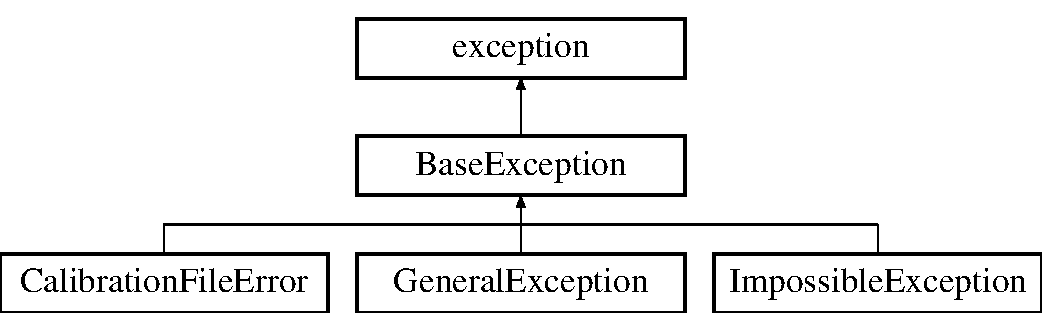
\includegraphics[height=3.000000cm]{class_base_exception}
\end{center}
\end{figure}
\subsection*{Public Member Functions}
\begin{DoxyCompactItemize}
\item 
\hypertarget{class_base_exception_a9a4668c1da76b424a113d600f313b67f}{virtual const char $\ast$ {\bfseries what} () const noexcept=0}\label{class_base_exception_a9a4668c1da76b424a113d600f313b67f}

\end{DoxyCompactItemize}


\subsection{Detailed Description}


Definition at line 10 of file base\-\_\-exception.\-h.



The documentation for this class was generated from the following files\-:\begin{DoxyCompactItemize}
\item 
/home/travis/build/tomas789/tonav/include/exceptions/base\-\_\-exception.\-h\item 
/home/travis/build/tomas789/tonav/src/exceptions/base\-\_\-exception.\-cpp\end{DoxyCompactItemize}

\hypertarget{class_calibration}{\section{Calibration Class Reference}
\label{class_calibration}\index{Calibration@{Calibration}}
}
\subsection*{Public Member Functions}
\begin{DoxyCompactItemize}
\item 
\hypertarget{class_calibration_a0273a577bae64d0833262103580e4a38}{int {\bfseries get\-Max\-Camera\-Poses} () const }\label{class_calibration_a0273a577bae64d0833262103580e4a38}

\item 
\hypertarget{class_calibration_acdf5d45d605b29f9114ae05600f07b76}{int {\bfseries get\-Buffer\-Size} () const }\label{class_calibration_acdf5d45d605b29f9114ae05600f07b76}

\item 
\hypertarget{class_calibration_a681582420d47807e4d8b1c8608e35aef}{int {\bfseries get\-Max\-Triangulation\-Iterations} () const }\label{class_calibration_a681582420d47807e4d8b1c8608e35aef}

\item 
\hypertarget{class_calibration_a871a481190b4ac5a4bb3ae1d5426726e}{Eigen\-::\-Matrix3d {\bfseries get\-Rotation\-From\-Body\-To\-Camera\-Frame} () const }\label{class_calibration_a871a481190b4ac5a4bb3ae1d5426726e}

\item 
\hypertarget{class_calibration_ad3edc4101a92835c6eed1dcfa004b592}{Eigen\-::\-Matrix$<$ double, 3, 3 $>$ {\bfseries get\-G\-Sensitivity\-Matrix} () const }\label{class_calibration_ad3edc4101a92835c6eed1dcfa004b592}

\item 
\hypertarget{class_calibration_a645b1a1cd460d493756669392ac71b78}{Eigen\-::\-Matrix$<$ double, 3, 3 $>$ {\bfseries get\-Gyroscope\-Shape\-Matrix} () const }\label{class_calibration_a645b1a1cd460d493756669392ac71b78}

\item 
\hypertarget{class_calibration_acd1d1fff6512b6fbfa8ff80cd45033f3}{Eigen\-::\-Matrix$<$ double, 3, 3 $>$ {\bfseries get\-Accelerometer\-Shape\-Matrix} () const }\label{class_calibration_acd1d1fff6512b6fbfa8ff80cd45033f3}

\item 
\hypertarget{class_calibration_a1144bc436545a52c5036ba6b02028c78}{Eigen\-::\-Matrix$<$ double, 3, 1 $>$ {\bfseries get\-Camera\-To\-Body\-Offset} () const }\label{class_calibration_a1144bc436545a52c5036ba6b02028c78}

\item 
\hypertarget{class_calibration_ab8e718f8167cbc0d15cb90983175ce9d}{double {\bfseries get\-Focal\-Length\-X} () const }\label{class_calibration_ab8e718f8167cbc0d15cb90983175ce9d}

\item 
\hypertarget{class_calibration_af25283fd143f9f8e4026afadff66188f}{double {\bfseries get\-Focal\-Length\-Y} () const }\label{class_calibration_af25283fd143f9f8e4026afadff66188f}

\item 
\hypertarget{class_calibration_aa101a7999e6eec103dce4ec651c2218b}{double {\bfseries get\-Optical\-Center\-X} () const }\label{class_calibration_aa101a7999e6eec103dce4ec651c2218b}

\item 
\hypertarget{class_calibration_a7486353559a45d424afb1aa6fbfa9f24}{double {\bfseries get\-Optical\-Center\-Y} () const }\label{class_calibration_a7486353559a45d424afb1aa6fbfa9f24}

\item 
\hypertarget{class_calibration_a57798a33c441afe2e0b675008e962af6}{Eigen\-::\-Matrix$<$ double, 3, 1 $>$ {\bfseries get\-Radial\-Distortion\-Parameters} () const }\label{class_calibration_a57798a33c441afe2e0b675008e962af6}

\item 
\hypertarget{class_calibration_ab42ba1d8120e3c22b85204c5dfd98f7f}{Eigen\-::\-Matrix$<$ double, 2, 1 $>$ {\bfseries get\-Tangential\-Distortion\-Parameters} () const }\label{class_calibration_ab42ba1d8120e3c22b85204c5dfd98f7f}

\item 
\hypertarget{class_calibration_a22c6544bba616210e34f9020479a32c6}{double {\bfseries get\-Camera\-Delay\-Time} () const }\label{class_calibration_a22c6544bba616210e34f9020479a32c6}

\item 
\hypertarget{class_calibration_aecbab0b6d724fa68f5af6e038111284b}{double {\bfseries get\-Camera\-Readout\-Time} () const }\label{class_calibration_aecbab0b6d724fa68f5af6e038111284b}

\end{DoxyCompactItemize}
\subsection*{Static Public Member Functions}
\begin{DoxyCompactItemize}
\item 
\hypertarget{class_calibration_a407d16502f36acfc7bd00572abe90739}{static \hyperlink{class_calibration}{Calibration} {\bfseries from\-Path} (boost\-::filesystem\-::path fname)}\label{class_calibration_a407d16502f36acfc7bd00572abe90739}

\item 
\hypertarget{class_calibration_a1d1c3b1b92ae75db9428f61b7afcc7f0}{static bool {\bfseries try\-Parse\-Int} (const std\-::string \&value, int \&out)}\label{class_calibration_a1d1c3b1b92ae75db9428f61b7afcc7f0}

\item 
\hypertarget{class_calibration_a043fc49ab017f6188dfb1b38cf7b573e}{static bool {\bfseries try\-Parse\-Double} (const std\-::string \&value, double \&out)}\label{class_calibration_a043fc49ab017f6188dfb1b38cf7b573e}

\item 
\hypertarget{class_calibration_a58c12342c94ea075107e6202e67c714a}{static bool {\bfseries try\-Parse\-Matrix3d} (const std\-::string \&value, Eigen\-::\-Matrix3d \&out)}\label{class_calibration_a58c12342c94ea075107e6202e67c714a}

\end{DoxyCompactItemize}


\subsection{Detailed Description}


Definition at line 13 of file calibration.\-h.



The documentation for this class was generated from the following files\-:\begin{DoxyCompactItemize}
\item 
/home/travis/build/tomas789/tonav/include/calibration.\-h\item 
/home/travis/build/tomas789/tonav/src/calibration.\-cpp\end{DoxyCompactItemize}

\hypertarget{class_calibration_file_error}{\section{Calibration\-File\-Error Class Reference}
\label{class_calibration_file_error}\index{Calibration\-File\-Error@{Calibration\-File\-Error}}
}
Inheritance diagram for Calibration\-File\-Error\-:\begin{figure}[H]
\begin{center}
\leavevmode
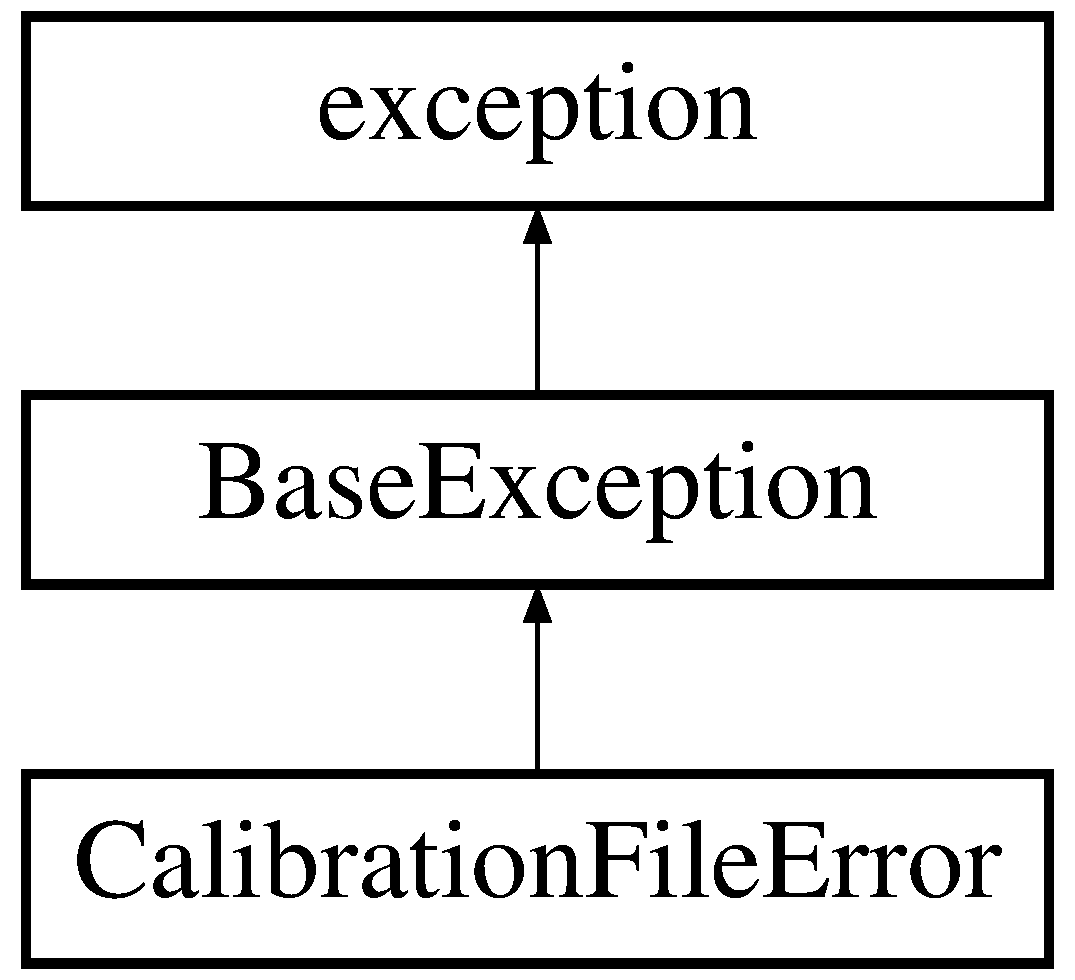
\includegraphics[height=3.000000cm]{class_calibration_file_error}
\end{center}
\end{figure}
\subsection*{Public Member Functions}
\begin{DoxyCompactItemize}
\item 
\hypertarget{class_calibration_file_error_ac4403a65bb13617f6f9aaea23a408c0a}{{\bfseries Calibration\-File\-Error} (const std\-::string \&msg)}\label{class_calibration_file_error_ac4403a65bb13617f6f9aaea23a408c0a}

\item 
\hypertarget{class_calibration_file_error_a91d41fb29208c4304760a251de8ca50a}{{\bfseries Calibration\-File\-Error} (int line\-\_\-number, const std\-::string \&msg)}\label{class_calibration_file_error_a91d41fb29208c4304760a251de8ca50a}

\item 
\hypertarget{class_calibration_file_error_a935a4e242a42bb1ab4867c05f44eebc9}{virtual const char $\ast$ {\bfseries what} () const noexcept}\label{class_calibration_file_error_a935a4e242a42bb1ab4867c05f44eebc9}

\end{DoxyCompactItemize}


\subsection{Detailed Description}


Definition at line 12 of file calibration\-\_\-file\-\_\-error.\-h.



The documentation for this class was generated from the following files\-:\begin{DoxyCompactItemize}
\item 
/home/tomaskrejci/catkin\-\_\-ws/src/tonav/include/exceptions/calibration\-\_\-file\-\_\-error.\-h\item 
/home/tomaskrejci/catkin\-\_\-ws/src/tonav/src/exceptions/calibration\-\_\-file\-\_\-error.\-cpp\end{DoxyCompactItemize}

\hypertarget{class_camera_feed}{\section{Camera\-Feed Class Reference}
\label{class_camera_feed}\index{Camera\-Feed@{Camera\-Feed}}
}
\subsection*{Public Member Functions}
\begin{DoxyCompactItemize}
\item 
\hypertarget{class_camera_feed_a2d7c8c329802b64568b312675115efce}{bool {\bfseries has\-Next} () const }\label{class_camera_feed_a2d7c8c329802b64568b312675115efce}

\item 
\hypertarget{class_camera_feed_a175a707efb56c2f3c78c2859129cbc24}{void {\bfseries next} ()}\label{class_camera_feed_a175a707efb56c2f3c78c2859129cbc24}

\item 
\hypertarget{class_camera_feed_ac703c1de71a7bf488f82921177ea4b0a}{const \hyperlink{class_camera_item}{Camera\-Item} \& {\bfseries top} () const }\label{class_camera_feed_ac703c1de71a7bf488f82921177ea4b0a}

\item 
\hypertarget{class_camera_feed_af761420a0337f52253b23c7d276516f8}{cv\-::\-Mat {\bfseries get\-Image} (const \hyperlink{class_camera_item}{Camera\-Item} \&item) const }\label{class_camera_feed_af761420a0337f52253b23c7d276516f8}

\end{DoxyCompactItemize}
\subsection*{Static Public Member Functions}
\begin{DoxyCompactItemize}
\item 
\hypertarget{class_camera_feed_a38c0ad4632b39babdc99fc65ddc56c36}{static \hyperlink{class_camera_feed}{Camera\-Feed} {\bfseries from\-Dataset} (boost\-::filesystem\-::path path)}\label{class_camera_feed_a38c0ad4632b39babdc99fc65ddc56c36}

\end{DoxyCompactItemize}


\subsection{Detailed Description}


Definition at line 18 of file camera\-\_\-feed.\-h.



The documentation for this class was generated from the following files\-:\begin{DoxyCompactItemize}
\item 
/home/travis/build/tomas789/tonav/include/camera\-\_\-feed.\-h\item 
/home/travis/build/tomas789/tonav/src/camera\-\_\-feed.\-cpp\end{DoxyCompactItemize}

\hypertarget{class_camera_item}{\section{Camera\-Item Class Reference}
\label{class_camera_item}\index{Camera\-Item@{Camera\-Item}}
}
\subsection*{Public Member Functions}
\begin{DoxyCompactItemize}
\item 
\hypertarget{class_camera_item_a6227ac10298e97b4ae86371de99cd4c9}{double {\bfseries get\-Time} () const }\label{class_camera_item_a6227ac10298e97b4ae86371de99cd4c9}

\item 
\hypertarget{class_camera_item_a6e19e5bdbfc691fb8abc4e94ef43f05e}{std\-::string {\bfseries get\-File\-Name} () const }\label{class_camera_item_a6e19e5bdbfc691fb8abc4e94ef43f05e}

\end{DoxyCompactItemize}
\subsection*{Static Public Member Functions}
\begin{DoxyCompactItemize}
\item 
\hypertarget{class_camera_item_a4cccf1e169a05288c47ecf232afb2086}{static \hyperlink{class_camera_item}{Camera\-Item} {\bfseries from\-String} (std\-::string fname)}\label{class_camera_item_a4cccf1e169a05288c47ecf232afb2086}

\end{DoxyCompactItemize}


\subsection{Detailed Description}


Definition at line 10 of file camera\-\_\-item.\-h.



The documentation for this class was generated from the following files\-:\begin{DoxyCompactItemize}
\item 
/home/travis/build/tomas789/tonav/include/camera\-\_\-item.\-h\item 
/home/travis/build/tomas789/tonav/src/camera\-\_\-item.\-cpp\end{DoxyCompactItemize}

\hypertarget{class_camera_pose}{\section{Camera\-Pose Class Reference}
\label{class_camera_pose}\index{Camera\-Pose@{Camera\-Pose}}
}
\subsection*{Public Types}
\begin{DoxyCompactItemize}
\item 
\hypertarget{class_camera_pose_a6898788bbfddfab4a5bf78d911477bf4}{using {\bfseries Camera\-Pose\-Type} = Eigen\-::\-Matrix$<$ double, 10, 1 $>$}\label{class_camera_pose_a6898788bbfddfab4a5bf78d911477bf4}

\end{DoxyCompactItemize}
\subsection*{Public Member Functions}
\begin{DoxyCompactItemize}
\item 
\hypertarget{class_camera_pose_a9393e875cfde4b1587a5f8b06d498466}{{\bfseries Camera\-Pose} (std\-::size\-\_\-t pose\-\_\-id)}\label{class_camera_pose_a9393e875cfde4b1587a5f8b06d498466}

\item 
\hypertarget{class_camera_pose_a91fe393ed7bd9c638198a7e138e3926c}{std\-::size\-\_\-t {\bfseries pose\-Id} () const }\label{class_camera_pose_a91fe393ed7bd9c638198a7e138e3926c}

\item 
\hypertarget{class_camera_pose_ab690a1975e061c75e2431c2f671d5637}{std\-::size\-\_\-t {\bfseries get\-Active\-Features\-Count} () const }\label{class_camera_pose_ab690a1975e061c75e2431c2f671d5637}

\item 
\hypertarget{class_camera_pose_ad52f534b1a0b4841a4c8d5e04471f0a1}{void {\bfseries set\-Active\-Features\-Count} (std\-::size\-\_\-t i)}\label{class_camera_pose_ad52f534b1a0b4841a4c8d5e04471f0a1}

\item 
\hypertarget{class_camera_pose_acfe976d10448deee4b714506c3ab6357}{void {\bfseries decrease\-Active\-Features\-Count} ()}\label{class_camera_pose_acfe976d10448deee4b714506c3ab6357}

\item 
\hypertarget{class_camera_pose_adeec70b16372d5aede066da2b6bf5d4a}{Eigen\-::\-Block$<$ Camera\-Pose\-Type, 4, 1 $>$ {\bfseries get\-Rotation\-For\-Body\-Pose\-Block} ()}\label{class_camera_pose_adeec70b16372d5aede066da2b6bf5d4a}

\item 
\hypertarget{class_camera_pose_af518728cc70c31460a20fc0f6f3f40a4}{Eigen\-::\-Block$<$ Camera\-Pose\-Type, 3, 1 $>$ {\bfseries get\-Position\-For\-Body\-Pose\-Block} ()}\label{class_camera_pose_af518728cc70c31460a20fc0f6f3f40a4}

\item 
\hypertarget{class_camera_pose_ae15933c2b5176d011135164962639a99}{Eigen\-::\-Block$<$ Camera\-Pose\-Type, 3, 1 $>$ {\bfseries get\-Velocity\-For\-Body\-Pose\-Block} ()}\label{class_camera_pose_ae15933c2b5176d011135164962639a99}

\item 
\hypertarget{class_camera_pose_aea5ef3206eb4f8929495dfc8f3a93571}{bool {\bfseries is\-Valid} () const }\label{class_camera_pose_aea5ef3206eb4f8929495dfc8f3a93571}

\end{DoxyCompactItemize}


\subsection{Detailed Description}


Definition at line 11 of file camera\-\_\-pose.\-h.



The documentation for this class was generated from the following files\-:\begin{DoxyCompactItemize}
\item 
/home/travis/build/tomas789/tonav/include/camera\-\_\-pose.\-h\item 
/home/travis/build/tomas789/tonav/src/camera\-\_\-pose.\-cpp\end{DoxyCompactItemize}

\hypertarget{class_feature_track}{\section{Feature\-Track Class Reference}
\label{class_feature_track}\index{Feature\-Track@{Feature\-Track}}
}
\subsection*{Public Member Functions}
\begin{DoxyCompactItemize}
\item 
\hypertarget{class_feature_track_ade7f659359480dab8f8ec7ace7625467}{{\bfseries Feature\-Track} (std\-::size\-\_\-t first\-\_\-frame\-\_\-number)}\label{class_feature_track_ade7f659359480dab8f8ec7ace7625467}

\item 
\hypertarget{class_feature_track_a5f13b226ac16fb0c9abe692c17f0f0c6}{void {\bfseries add\-Feature\-Position} (double x, double y)}\label{class_feature_track_a5f13b226ac16fb0c9abe692c17f0f0c6}

\item 
\hypertarget{class_feature_track_aa21cd2b1af1f2aaea1e7d19631f80474}{void {\bfseries revert\-Last\-Position} ()}\label{class_feature_track_aa21cd2b1af1f2aaea1e7d19631f80474}

\item 
\hypertarget{class_feature_track_a1635683732cdfda103a37d926d2efbf9}{std\-::size\-\_\-t {\bfseries get\-First\-Frame\-Number} () const }\label{class_feature_track_a1635683732cdfda103a37d926d2efbf9}

\item 
\hypertarget{class_feature_track_a966f8f018b7305d764216880f4a6f8ba}{bool {\bfseries is\-Out\-Of\-View} () const }\label{class_feature_track_a966f8f018b7305d764216880f4a6f8ba}

\item 
\hypertarget{class_feature_track_a75a507f6ac11d3a9319523d131c7949d}{void {\bfseries set\-Out\-Of\-View} ()}\label{class_feature_track_a75a507f6ac11d3a9319523d131c7949d}

\end{DoxyCompactItemize}


\subsection{Detailed Description}


Definition at line 11 of file feature\-\_\-track.\-h.



The documentation for this class was generated from the following files\-:\begin{DoxyCompactItemize}
\item 
/home/travis/build/tomas789/tonav/include/feature\-\_\-track.\-h\item 
/home/travis/build/tomas789/tonav/src/feature\-\_\-track.\-cpp\end{DoxyCompactItemize}

\hypertarget{class_feature_tracker}{\section{Feature\-Tracker Class Reference}
\label{class_feature_tracker}\index{Feature\-Tracker@{Feature\-Tracker}}
}
\subsection*{Public Types}
\begin{DoxyCompactItemize}
\item 
\hypertarget{class_feature_tracker_a8c26ba2ee4c3653c6082a6ceec345f8a}{using {\bfseries feature\-\_\-track\-\_\-list} = std\-::vector$<$ std\-::shared\-\_\-ptr$<$ \hyperlink{class_feature_track}{Feature\-Track} $>$$>$}\label{class_feature_tracker_a8c26ba2ee4c3653c6082a6ceec345f8a}

\end{DoxyCompactItemize}
\subsection*{Public Member Functions}
\begin{DoxyCompactItemize}
\item 
\hypertarget{class_feature_tracker_a1d44cc6cd06ced4f321d2ecebfd7b069}{feature\-\_\-track\-\_\-list {\bfseries process\-Image} (feature\-\_\-track\-\_\-list \&previous\-\_\-tracks, cv\-::\-Mat \&image)}\label{class_feature_tracker_a1d44cc6cd06ced4f321d2ecebfd7b069}

\end{DoxyCompactItemize}


\subsection{Detailed Description}


Definition at line 15 of file feature\-\_\-tracker.\-h.



The documentation for this class was generated from the following files\-:\begin{DoxyCompactItemize}
\item 
/home/tomaskrejci/catkin\-\_\-ws/src/tonav/include/feature\-\_\-tracker.\-h\item 
/home/tomaskrejci/catkin\-\_\-ws/src/tonav/src/feature\-\_\-tracker.\-cpp\end{DoxyCompactItemize}

\hypertarget{class_filter}{\section{Filter Class Reference}
\label{class_filter}\index{Filter@{Filter}}
}


Implementation of M\-S\-C\-K\-F.  




{\ttfamily \#include $<$filter.\-h$>$}

\subsection*{Public Member Functions}
\begin{DoxyCompactItemize}
\item 
\hypertarget{class_filter_ac00d9ce620e60b2c8b26ca9cad7e1b39}{{\bfseries Filter} (const \hyperlink{class_calibration}{Calibration} \&calibration)}\label{class_filter_ac00d9ce620e60b2c8b26ca9cad7e1b39}

\item 
\hypertarget{class_filter_a5742b1247b9f92a9148d99386cdd3876}{void {\bfseries initialize} ()}\label{class_filter_a5742b1247b9f92a9148d99386cdd3876}

\item 
\hypertarget{class_filter_a27176eb65976f98cdc9495b4fdfc3296}{void {\bfseries step\-Inertial} (double timedelta, const \hyperlink{class_imu_item}{Imu\-Item} \&accel, const \hyperlink{class_imu_item}{Imu\-Item} \&gyro)}\label{class_filter_a27176eb65976f98cdc9495b4fdfc3296}

\item 
\hypertarget{class_filter_a1fad49c62892905f713de0bf66d9f3c7}{void {\bfseries step\-Camera} (double timedelta, const \hyperlink{class_imu_item}{Imu\-Item} \&accel, const \hyperlink{class_imu_item}{Imu\-Item} \&gyro, cv\-::\-Mat \&frame)}\label{class_filter_a1fad49c62892905f713de0bf66d9f3c7}

\item 
\hypertarget{class_filter_a3ed7acd6fff45ead8b4209d4e31a8097}{void {\bfseries propagate\-Rotation} (\hyperlink{class_filter_state}{Filter\-State} \&old\-\_\-state, \hyperlink{class_filter_state}{Filter\-State} \&new\-\_\-state, double timedelta, const \hyperlink{class_imu_item}{Imu\-Item} \&accel, const \hyperlink{class_imu_item}{Imu\-Item} \&gyro)}\label{class_filter_a3ed7acd6fff45ead8b4209d4e31a8097}

\item 
\hypertarget{class_filter_a778f444068abe887fd58e02f00be6121}{void {\bfseries propagate\-Velocity\-And\-Position} (\hyperlink{class_filter_state}{Filter\-State} \&old\-\_\-state, \hyperlink{class_filter_state}{Filter\-State} \&new\-\_\-state, double timedelta, const \hyperlink{class_imu_item}{Imu\-Item} \&accel, const \hyperlink{class_imu_item}{Imu\-Item} \&gyro)}\label{class_filter_a778f444068abe887fd58e02f00be6121}

\item 
void \hyperlink{class_filter_ad046b83209a1f03d65ac75f16b538546}{set\-Global\-Gravity} (Eigen\-::\-Vector3d gravity)
\begin{DoxyCompactList}\small\item\em Set initial estimate of gravity in global frame. \end{DoxyCompactList}\item 
\hypertarget{class_filter_aeeb0c2e971a47c73c2f950aa8890f1ac}{Eigen\-::\-Vector3d {\bfseries get\-Global\-Gravity} () const }\label{class_filter_aeeb0c2e971a47c73c2f950aa8890f1ac}

\item 
\hypertarget{class_filter_a936ea0f9f4f587d0cd9bc26a4a73df34}{Eigen\-::\-Vector3d {\bfseries get\-Current\-Position} ()}\label{class_filter_a936ea0f9f4f587d0cd9bc26a4a73df34}

\item 
\hypertarget{class_filter_a7094e57e502a4fc7f124f0d1184eb133}{Eigen\-::\-Quaterniond {\bfseries get\-Current\-Attitude} ()}\label{class_filter_a7094e57e502a4fc7f124f0d1184eb133}

\item 
double \hyperlink{class_filter_a1c7a33a737fafec46d6e98ec1be37a4c}{get\-Image\-Capture\-Time} (double arrive\-\_\-time)
\begin{DoxyCompactList}\small\item\em Calculate $\hat{t} = t + \hat{t}_d$. \end{DoxyCompactList}\end{DoxyCompactItemize}


\subsection{Detailed Description}
Implementation of M\-S\-C\-K\-F. 

This is core functionality of \hyperlink{class_tonav}{Tonav}. All methods must be called with caution. It assumes correct order of update steps.

Don't use this class directly. Use \hyperlink{class_tonav}{Tonav} or \hyperlink{class_tonav_ros}{Tonav\-Ros} instead 

Definition at line 29 of file filter.\-h.



\subsection{Member Function Documentation}
\hypertarget{class_filter_a1c7a33a737fafec46d6e98ec1be37a4c}{\index{Filter@{Filter}!get\-Image\-Capture\-Time@{get\-Image\-Capture\-Time}}
\index{get\-Image\-Capture\-Time@{get\-Image\-Capture\-Time}!Filter@{Filter}}
\subsubsection[{get\-Image\-Capture\-Time}]{\setlength{\rightskip}{0pt plus 5cm}double Filter\-::get\-Image\-Capture\-Time (
\begin{DoxyParamCaption}
\item[{double}]{arrive\-\_\-time}
\end{DoxyParamCaption}
)}}\label{class_filter_a1c7a33a737fafec46d6e98ec1be37a4c}


Calculate $\hat{t} = t + \hat{t}_d$. 

This method calculates image capture time from time when image arrived.


\begin{DoxyParams}{Parameters}
{\em arrive\-\_\-time} & Time whan image arrived \\
\hline
\end{DoxyParams}
\begin{DoxyReturn}{Returns}
Estimated image capture time 
\end{DoxyReturn}


Definition at line 142 of file filter.\-cpp.

\hypertarget{class_filter_ad046b83209a1f03d65ac75f16b538546}{\index{Filter@{Filter}!set\-Global\-Gravity@{set\-Global\-Gravity}}
\index{set\-Global\-Gravity@{set\-Global\-Gravity}!Filter@{Filter}}
\subsubsection[{set\-Global\-Gravity}]{\setlength{\rightskip}{0pt plus 5cm}void Filter\-::set\-Global\-Gravity (
\begin{DoxyParamCaption}
\item[{Eigen\-::\-Vector3d}]{gravity}
\end{DoxyParamCaption}
)}}\label{class_filter_ad046b83209a1f03d65ac75f16b538546}


Set initial estimate of gravity in global frame. 

This is usually calculated as averate of first few accelerometer measurements. It assumes, that device don't move for few seconds at the beginning.


\begin{DoxyParams}{Parameters}
{\em gravity} & Initial estimate of gravity in global frame. \\
\hline
\end{DoxyParams}


Definition at line 126 of file filter.\-cpp.



The documentation for this class was generated from the following files\-:\begin{DoxyCompactItemize}
\item 
/home/travis/build/tomas789/tonav/include/filter.\-h\item 
/home/travis/build/tomas789/tonav/src/filter.\-cpp\end{DoxyCompactItemize}

\hypertarget{class_filter_state}{\section{Filter\-State Class Reference}
\label{class_filter_state}\index{Filter\-State@{Filter\-State}}
}
\subsection*{Public Types}
\begin{DoxyCompactItemize}
\item 
\hypertarget{class_filter_state_a26539bef949b11d11deb68ab8fba5598}{using {\bfseries State\-Type} = Eigen\-::\-Matrix$<$ double, 57, 1 $>$}\label{class_filter_state_a26539bef949b11d11deb68ab8fba5598}

\end{DoxyCompactItemize}
\subsection*{Public Member Functions}
\begin{DoxyCompactItemize}
\item 
\hypertarget{class_filter_state_a549088ec74cb2262e397b929abc174d2}{Eigen\-::\-Block$<$ State\-Type, 4, 1 $>$ {\bfseries get\-Rotation\-Block} ()}\label{class_filter_state_a549088ec74cb2262e397b929abc174d2}

\item 
\hypertarget{class_filter_state_a5f61beb08bf43811cebea645c80949ac}{Eigen\-::\-Quaterniond {\bfseries get\-Rotation\-Quaternion} ()}\label{class_filter_state_a5f61beb08bf43811cebea645c80949ac}

\item 
\hypertarget{class_filter_state_ab2a6e477d01da9521267781a73757838}{void {\bfseries set\-Rotation\-Quaternion} (const Eigen\-::\-Quaterniond \&quat)}\label{class_filter_state_ab2a6e477d01da9521267781a73757838}

\item 
\hypertarget{class_filter_state_af2dd9af9a0722a05cbc59981cf40aead}{Eigen\-::\-Block$<$ State\-Type, 3, 1 $>$ {\bfseries get\-Position\-Block} ()}\label{class_filter_state_af2dd9af9a0722a05cbc59981cf40aead}

\item 
\hypertarget{class_filter_state_a239c2732f1a3d647c21b96f5d53dd215}{Eigen\-::\-Block$<$ State\-Type, 3, 1 $>$ {\bfseries get\-Velocity\-Block} ()}\label{class_filter_state_a239c2732f1a3d647c21b96f5d53dd215}

\item 
\hypertarget{class_filter_state_a43b485d8c02d6eb8e37cd8f2323e9e43}{Eigen\-::\-Block$<$ State\-Type, 3, 1 $>$ {\bfseries get\-Accelerometer\-Bias\-Block} ()}\label{class_filter_state_a43b485d8c02d6eb8e37cd8f2323e9e43}

\item 
\hypertarget{class_filter_state_a8bb562801b8b34026dad74bd4223c06e}{Eigen\-::\-Block$<$ State\-Type, 3, 1 $>$ {\bfseries get\-Gyroscope\-Bias\-Block} ()}\label{class_filter_state_a8bb562801b8b34026dad74bd4223c06e}

\item 
\hypertarget{class_filter_state_a8686bb8e54e2e9902c28095f8c623745}{Eigen\-::\-Block$<$ State\-Type, 9, 1 $>$ {\bfseries get\-Gyroscope\-Shape\-Vectorized\-Block} ()}\label{class_filter_state_a8686bb8e54e2e9902c28095f8c623745}

\item 
\hypertarget{class_filter_state_a1ab46a729807178faf9b6bebb87aa791}{Eigen\-::\-Block$<$ State\-Type, 9, 1 $>$ {\bfseries get\-G\-Sensitivity\-Vectorized\-Block} ()}\label{class_filter_state_a1ab46a729807178faf9b6bebb87aa791}

\item 
\hypertarget{class_filter_state_a57cb64b2b25132c2da38b0313da415c5}{Eigen\-::\-Block$<$ State\-Type, 9, 1 $>$ {\bfseries get\-Accelerometer\-Shape\-Vectorized\-Block} ()}\label{class_filter_state_a57cb64b2b25132c2da38b0313da415c5}

\item 
\hypertarget{class_filter_state_a844855f0fa5ebf0c606a06ea6fdb460b}{Eigen\-::\-Block$<$ State\-Type, 3, 1 $>$ {\bfseries get\-Camera\-To\-Body\-Offset\-Block} ()}\label{class_filter_state_a844855f0fa5ebf0c606a06ea6fdb460b}

\item 
\hypertarget{class_filter_state_a3b65a9649366c853ffd99784fe9bef72}{double \& {\bfseries get\-Focal\-Length\-X\-Ref} ()}\label{class_filter_state_a3b65a9649366c853ffd99784fe9bef72}

\item 
\hypertarget{class_filter_state_aed71d6cec7d8a101ba10b83f969d28d4}{double \& {\bfseries get\-Focal\-Length\-Y\-Ref} ()}\label{class_filter_state_aed71d6cec7d8a101ba10b83f969d28d4}

\item 
\hypertarget{class_filter_state_a3fc41a17c48851340acbfdfc9c164f01}{double \& {\bfseries get\-Optical\-Center\-X\-Ref} ()}\label{class_filter_state_a3fc41a17c48851340acbfdfc9c164f01}

\item 
\hypertarget{class_filter_state_a7ddf9eca9ab6cad9bee85ee6cfc80de0}{double \& {\bfseries get\-Optical\-Center\-Y\-Ref} ()}\label{class_filter_state_a7ddf9eca9ab6cad9bee85ee6cfc80de0}

\item 
\hypertarget{class_filter_state_aa326b846da2b55623e4d219d357e6b57}{Eigen\-::\-Block$<$ State\-Type, 3, 1 $>$ {\bfseries get\-Radial\-Distortion\-Parameters\-Block} ()}\label{class_filter_state_aa326b846da2b55623e4d219d357e6b57}

\item 
\hypertarget{class_filter_state_ad4b9c49509f2cc303c554969a8264c89}{Eigen\-::\-Block$<$ State\-Type, 2, 1 $>$ {\bfseries get\-Tangential\-Distortion\-Parameters\-Block} ()}\label{class_filter_state_ad4b9c49509f2cc303c554969a8264c89}

\item 
\hypertarget{class_filter_state_a6563a73bad1016317018c85d53380962}{double \& {\bfseries get\-Camera\-Delay\-Time\-Ref} ()}\label{class_filter_state_a6563a73bad1016317018c85d53380962}

\item 
\hypertarget{class_filter_state_ab9d3e7cad1ae09ed35bcc528c0e8ef45}{double \& {\bfseries get\-Camera\-Readout\-Time\-Ref} ()}\label{class_filter_state_ab9d3e7cad1ae09ed35bcc528c0e8ef45}

\item 
\hypertarget{class_filter_state_a928bd10a77b39859d6f108f8dd8ae0e9}{Eigen\-::\-Block$<$ Eigen\-::\-Vector3d, 3, 1 $>$ {\bfseries get\-Rotation\-Estimate\-Block} ()}\label{class_filter_state_a928bd10a77b39859d6f108f8dd8ae0e9}

\item 
\hypertarget{class_filter_state_a4436166f7dbaf6c002b6fc2832b4f136}{Eigen\-::\-Block$<$ Eigen\-::\-Vector3d, 3, 1 $>$ {\bfseries get\-Acceleration\-Estimate\-Block} ()}\label{class_filter_state_a4436166f7dbaf6c002b6fc2832b4f136}

\item 
\hypertarget{class_filter_state_ab3d02580cdbd89bc64276467d7c1c854}{Eigen\-::\-Quaterniond {\bfseries get\-Rotation\-To\-This\-Frame} ()}\label{class_filter_state_ab3d02580cdbd89bc64276467d7c1c854}

\item 
\hypertarget{class_filter_state_ae820e97a5a74c7765780bc7bb223796b}{void {\bfseries set\-Rotation\-To\-This\-Frame} (const Eigen\-::\-Quaterniond \&quat)}\label{class_filter_state_ae820e97a5a74c7765780bc7bb223796b}

\item 
\hypertarget{class_filter_state_aed4aab3a5133d37924bc5c1284b6cb66}{std\-::ostream \& {\bfseries ugly\-Print} (std\-::ostream \&out) const }\label{class_filter_state_aed4aab3a5133d37924bc5c1284b6cb66}

\item 
\hypertarget{class_filter_state_af33cfbc67284846e3ca9c26a79c227a9}{\hyperlink{class_filter_state}{Filter\-State} {\bfseries derive\-New\-State\-For\-Imu\-Propagation} () const }\label{class_filter_state_af33cfbc67284846e3ca9c26a79c227a9}

\item 
\hypertarget{class_filter_state_a9fdc71df11cf72369b86be2eaffcea27}{void {\bfseries append\-Camera\-Pose} (const \hyperlink{class_camera_pose}{Camera\-Pose} \&camera\-\_\-pose)}\label{class_filter_state_a9fdc71df11cf72369b86be2eaffcea27}

\end{DoxyCompactItemize}


\subsection{Detailed Description}


Definition at line 14 of file filter\-\_\-state.\-h.



The documentation for this class was generated from the following files\-:\begin{DoxyCompactItemize}
\item 
/home/tomaskrejci/catkin\-\_\-ws/src/tonav/include/filter\-\_\-state.\-h\item 
/home/tomaskrejci/catkin\-\_\-ws/src/tonav/src/filter\-\_\-state.\-cpp\end{DoxyCompactItemize}

\hypertarget{class_frame_features}{\section{Frame\-Features Class Reference}
\label{class_frame_features}\index{Frame\-Features@{Frame\-Features}}
}
\subsection*{Public Member Functions}
\begin{DoxyCompactItemize}
\item 
\hypertarget{class_frame_features_a6977a4effbe856ff8583f4352cd138b8}{std\-::vector$<$ cv\-::\-D\-Match $>$ {\bfseries match} (cv\-::\-Ptr$<$ cv\-::\-Descriptor\-Matcher $>$ matcher, const \hyperlink{class_frame_features}{Frame\-Features} \&other)}\label{class_frame_features_a6977a4effbe856ff8583f4352cd138b8}

\item 
\hypertarget{class_frame_features_ae36e05c015c5980fb0801fc0b6ee97ca}{void {\bfseries draw\-Features} (cv\-::\-Mat \&image, cv\-::\-Scalar color=cv\-::\-Scalar(255, 0, 0))}\label{class_frame_features_ae36e05c015c5980fb0801fc0b6ee97ca}

\item 
\hypertarget{class_frame_features_aff3c47e301fde7db68ecac5d852c6edf}{std\-::vector$<$ cv\-::\-Key\-Point $>$ \& {\bfseries keypoints} ()}\label{class_frame_features_aff3c47e301fde7db68ecac5d852c6edf}

\item 
\hypertarget{class_frame_features_a29b51fc67b07fe6e5b9236a092d1e17a}{const std\-::vector$<$ cv\-::\-Key\-Point $>$ \& {\bfseries keypoints} () const }\label{class_frame_features_a29b51fc67b07fe6e5b9236a092d1e17a}

\end{DoxyCompactItemize}
\subsection*{Static Public Member Functions}
\begin{DoxyCompactItemize}
\item 
\hypertarget{class_frame_features_a5942b53a2e105a82e6454cd259157aa0}{static \hyperlink{class_frame_features}{Frame\-Features} {\bfseries from\-Image} (cv\-::\-Ptr$<$ cv\-::\-Feature\-Detector $>$ detector, cv\-::\-Ptr$<$ cv\-::\-Descriptor\-Extractor $>$ extractor, cv\-::\-Mat \&image)}\label{class_frame_features_a5942b53a2e105a82e6454cd259157aa0}

\end{DoxyCompactItemize}


\subsection{Detailed Description}


Definition at line 11 of file frame\-\_\-features.\-h.



The documentation for this class was generated from the following files\-:\begin{DoxyCompactItemize}
\item 
/home/travis/build/tomas789/tonav/include/frame\-\_\-features.\-h\item 
/home/travis/build/tomas789/tonav/src/frame\-\_\-features.\-cpp\end{DoxyCompactItemize}

\hypertarget{class_general_exception}{\section{General\-Exception Class Reference}
\label{class_general_exception}\index{General\-Exception@{General\-Exception}}
}
Inheritance diagram for General\-Exception\-:\begin{figure}[H]
\begin{center}
\leavevmode
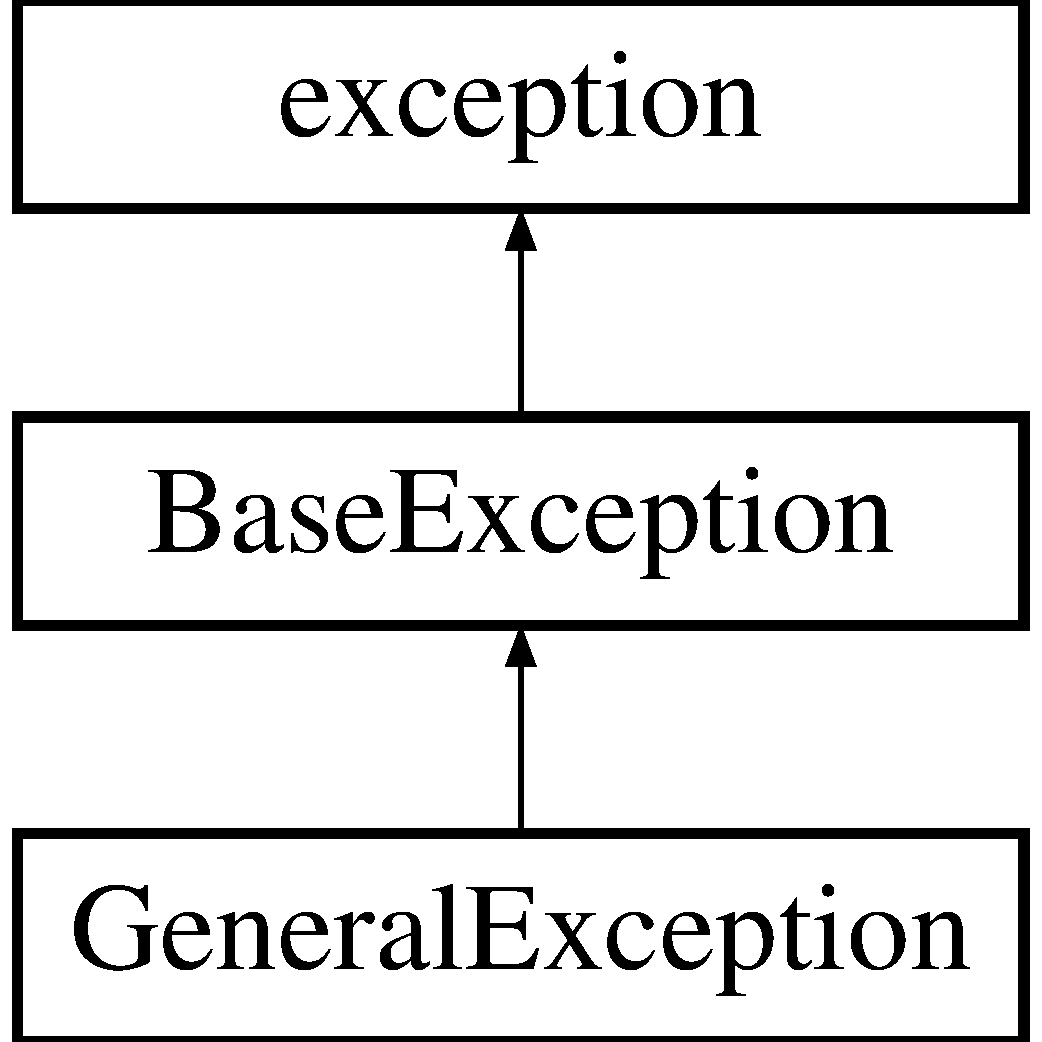
\includegraphics[height=3.000000cm]{class_general_exception}
\end{center}
\end{figure}
\subsection*{Public Member Functions}
\begin{DoxyCompactItemize}
\item 
\hypertarget{class_general_exception_ae9a9599d82aa29bef098dbb594e2f13e}{{\bfseries General\-Exception} (const std\-::string \&msg)}\label{class_general_exception_ae9a9599d82aa29bef098dbb594e2f13e}

\item 
\hypertarget{class_general_exception_ab6bb7c8ae3ab248e082d7fbf3f4a2cf3}{{\bfseries General\-Exception} (int line\-\_\-number, const std\-::string \&msg)}\label{class_general_exception_ab6bb7c8ae3ab248e082d7fbf3f4a2cf3}

\item 
\hypertarget{class_general_exception_a1d8d27063e77fe4658daa8279d0af52c}{virtual const char $\ast$ {\bfseries what} () const noexcept}\label{class_general_exception_a1d8d27063e77fe4658daa8279d0af52c}

\end{DoxyCompactItemize}


\subsection{Detailed Description}


Definition at line 12 of file general\-\_\-exception.\-h.



The documentation for this class was generated from the following files\-:\begin{DoxyCompactItemize}
\item 
/home/tomaskrejci/catkin\-\_\-ws/src/tonav/include/exceptions/general\-\_\-exception.\-h\item 
/home/tomaskrejci/catkin\-\_\-ws/src/tonav/src/exceptions/general\-\_\-exception.\-cpp\end{DoxyCompactItemize}

\hypertarget{class_impossible_exception}{\section{Impossible\-Exception Class Reference}
\label{class_impossible_exception}\index{Impossible\-Exception@{Impossible\-Exception}}
}
Inheritance diagram for Impossible\-Exception\-:\begin{figure}[H]
\begin{center}
\leavevmode
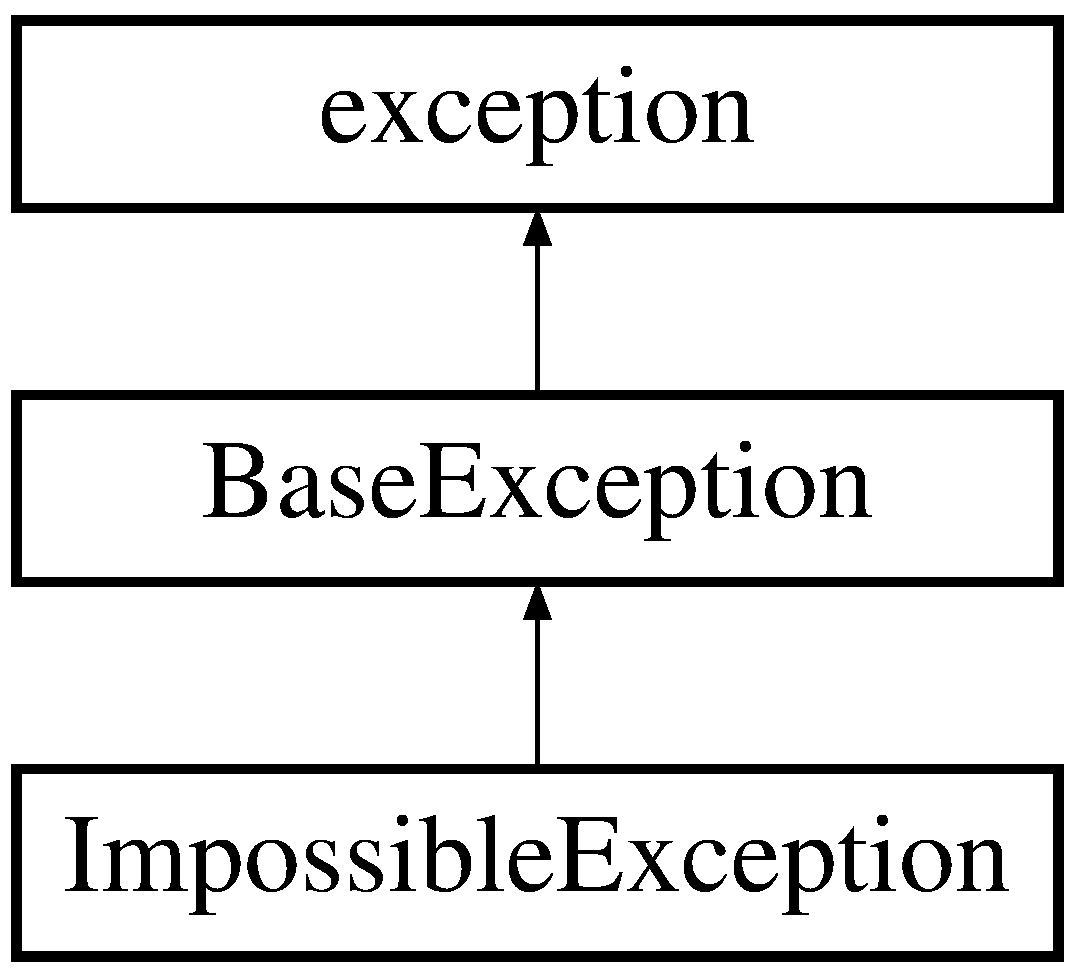
\includegraphics[height=3.000000cm]{class_impossible_exception}
\end{center}
\end{figure}
\subsection*{Public Member Functions}
\begin{DoxyCompactItemize}
\item 
\hypertarget{class_impossible_exception_a88afecc506123920b1bcd8f8b1bc612d}{{\bfseries Impossible\-Exception} (const std\-::string \&msg)}\label{class_impossible_exception_a88afecc506123920b1bcd8f8b1bc612d}

\item 
\hypertarget{class_impossible_exception_a3368d553e27e69451266f56bc37e9a86}{virtual const char $\ast$ {\bfseries what} () const noexcept}\label{class_impossible_exception_a3368d553e27e69451266f56bc37e9a86}

\end{DoxyCompactItemize}


\subsection{Detailed Description}


Definition at line 12 of file impossible\-\_\-exception.\-h.



The documentation for this class was generated from the following files\-:\begin{DoxyCompactItemize}
\item 
/home/travis/build/tomas789/tonav/include/exceptions/impossible\-\_\-exception.\-h\item 
/home/travis/build/tomas789/tonav/src/exceptions/impossible\-\_\-exception.\-cpp\end{DoxyCompactItemize}

\hypertarget{class_imu_buffer}{\section{Imu\-Buffer Class Reference}
\label{class_imu_buffer}\index{Imu\-Buffer@{Imu\-Buffer}}
}


Buffer of I\-M\-U data measurements.  




{\ttfamily \#include $<$imu\-\_\-buffer.\-h$>$}

\subsection*{Public Member Functions}
\begin{DoxyCompactItemize}
\item 
\hypertarget{class_imu_buffer_a50dd06412b4e7f3f041ae6ab6fa680b0}{{\bfseries Imu\-Buffer} (Imu\-Device device, std\-::size\-\_\-t size)}\label{class_imu_buffer_a50dd06412b4e7f3f041ae6ab6fa680b0}

\item 
\hypertarget{class_imu_buffer_a03aff5b4ab113232a3fa032115249018}{void {\bfseries add\-Measurement} (\hyperlink{class_imu_item}{Imu\-Item} item)}\label{class_imu_buffer_a03aff5b4ab113232a3fa032115249018}

\item 
\hypertarget{class_imu_buffer_a70e3b571c1ff9c9e2ca60c8dfd1eee1c}{\hyperlink{class_imu_item}{Imu\-Item} {\bfseries interpolate\-At\-Time} (double time) const }\label{class_imu_buffer_a70e3b571c1ff9c9e2ca60c8dfd1eee1c}

\item 
\hypertarget{class_imu_buffer_a3c23315625f26a5673b814f513c1bc98}{double {\bfseries get\-Min\-Time} () const }\label{class_imu_buffer_a3c23315625f26a5673b814f513c1bc98}

\item 
\hypertarget{class_imu_buffer_aa3f3a11dc21d97386b3154122cb8e296}{double {\bfseries get\-Max\-Time} () const }\label{class_imu_buffer_aa3f3a11dc21d97386b3154122cb8e296}

\item 
\hypertarget{class_imu_buffer_a4500c72f04ac02e629e77762953c6abc}{bool {\bfseries is\-Ready} () const }\label{class_imu_buffer_a4500c72f04ac02e629e77762953c6abc}

\end{DoxyCompactItemize}


\subsection{Detailed Description}
Buffer of I\-M\-U data measurements. 

\begin{DoxyRefDesc}{Deprecated}
\item[\hyperlink{deprecated__deprecated000002}{Deprecated}]This class is no longer needed. It is used in \hyperlink{class_navigator}{Navigator} class only.\end{DoxyRefDesc}


Using this class you can interpolate I\-M\-U measurement at any time in interval \mbox{[}get\-Min\-Time(), get\-Max\-Time()\mbox{]} 

Definition at line 22 of file imu\-\_\-buffer.\-h.



The documentation for this class was generated from the following files\-:\begin{DoxyCompactItemize}
\item 
/home/travis/build/tomas789/tonav/include/imu\-\_\-buffer.\-h\item 
/home/travis/build/tomas789/tonav/src/imu\-\_\-buffer.\-cpp\end{DoxyCompactItemize}

\hypertarget{class_imu_feed}{\section{Imu\-Feed Class Reference}
\label{class_imu_feed}\index{Imu\-Feed@{Imu\-Feed}}
}
\subsection*{Public Member Functions}
\begin{DoxyCompactItemize}
\item 
\hypertarget{class_imu_feed_a5ab48b9002ee9eacfe760afc579e1b50}{bool {\bfseries has\-Next} () const }\label{class_imu_feed_a5ab48b9002ee9eacfe760afc579e1b50}

\item 
\hypertarget{class_imu_feed_ab36b0a9833d5687820065483818de270}{void {\bfseries next} ()}\label{class_imu_feed_ab36b0a9833d5687820065483818de270}

\item 
\hypertarget{class_imu_feed_a48e5bf07fb20dc5f55e3078b6c57adc2}{const \hyperlink{class_imu_item}{Imu\-Item} \& {\bfseries top} () const }\label{class_imu_feed_a48e5bf07fb20dc5f55e3078b6c57adc2}

\end{DoxyCompactItemize}
\subsection*{Static Public Member Functions}
\begin{DoxyCompactItemize}
\item 
\hypertarget{class_imu_feed_a65c5b70f27e938f6a13bd55fd0bb5127}{static \hyperlink{class_imu_feed}{Imu\-Feed} {\bfseries from\-Dataset} (boost\-::filesystem\-::path path)}\label{class_imu_feed_a65c5b70f27e938f6a13bd55fd0bb5127}

\end{DoxyCompactItemize}


\subsection{Detailed Description}


Definition at line 14 of file imu\-\_\-feed.\-h.



The documentation for this class was generated from the following files\-:\begin{DoxyCompactItemize}
\item 
/home/travis/build/tomas789/tonav/include/imu\-\_\-feed.\-h\item 
/home/travis/build/tomas789/tonav/src/imu\-\_\-feed.\-cpp\end{DoxyCompactItemize}

\hypertarget{class_imu_item}{\section{Imu\-Item Class Reference}
\label{class_imu_item}\index{Imu\-Item@{Imu\-Item}}
}
\subsection*{Public Member Functions}
\begin{DoxyCompactItemize}
\item 
\hypertarget{class_imu_item_ac12a9c7f77a7318de5893a26284c8f12}{Imu\-Device {\bfseries get\-Device} () const }\label{class_imu_item_ac12a9c7f77a7318de5893a26284c8f12}

\item 
\hypertarget{class_imu_item_adf0603391765e4950651ee67fe2273b7}{double {\bfseries get\-Time} () const }\label{class_imu_item_adf0603391765e4950651ee67fe2273b7}

\item 
\hypertarget{class_imu_item_a9fe54cf71ea23dc3f044bf849a50743b}{double {\bfseries get\-X} () const }\label{class_imu_item_a9fe54cf71ea23dc3f044bf849a50743b}

\item 
\hypertarget{class_imu_item_af969726f713eb67b6b544133bea5fd21}{double {\bfseries get\-Y} () const }\label{class_imu_item_af969726f713eb67b6b544133bea5fd21}

\item 
\hypertarget{class_imu_item_af010fd2fd5ecd5868764a760f6040af5}{double {\bfseries get\-Z} () const }\label{class_imu_item_af010fd2fd5ecd5868764a760f6040af5}

\item 
\hypertarget{class_imu_item_a1cd4668ce368cb3b8360f42a1ab97580}{Eigen\-::\-Vector3d {\bfseries get\-Vector} () const }\label{class_imu_item_a1cd4668ce368cb3b8360f42a1ab97580}

\end{DoxyCompactItemize}
\subsection*{Static Public Member Functions}
\begin{DoxyCompactItemize}
\item 
\hypertarget{class_imu_item_af127ca299205f31693ed6a85330bf915}{static \hyperlink{class_imu_item}{Imu\-Item} {\bfseries from\-String} (std\-::string line)}\label{class_imu_item_af127ca299205f31693ed6a85330bf915}

\item 
\hypertarget{class_imu_item_a0a28edeccaf5f42fabf05e76c5c46519}{static \hyperlink{class_imu_item}{Imu\-Item} {\bfseries from\-Vector3d} (double time, const Imu\-Device \&device, const Eigen\-::\-Vector3d \&data)}\label{class_imu_item_a0a28edeccaf5f42fabf05e76c5c46519}

\end{DoxyCompactItemize}
\subsection*{Friends}
\begin{DoxyCompactItemize}
\item 
\hypertarget{class_imu_item_affcdaeabb9b33248d9efdf687f2eab5c}{class {\bfseries Imu\-Buffer}}\label{class_imu_item_affcdaeabb9b33248d9efdf687f2eab5c}

\end{DoxyCompactItemize}


\subsection{Detailed Description}


Definition at line 15 of file imu\-\_\-item.\-h.



The documentation for this class was generated from the following files\-:\begin{DoxyCompactItemize}
\item 
/home/tomaskrejci/catkin\-\_\-ws/src/tonav/include/imu\-\_\-item.\-h\item 
/home/tomaskrejci/catkin\-\_\-ws/src/tonav/src/imu\-\_\-item.\-cpp\end{DoxyCompactItemize}

\hypertarget{class_navigator}{\section{Navigator Class Reference}
\label{class_navigator}\index{Navigator@{Navigator}}
}


Perform navigation from dataset.  




{\ttfamily \#include $<$navigator.\-h$>$}

\subsection*{Public Member Functions}
\begin{DoxyCompactItemize}
\item 
int \hyperlink{class_navigator_a614e53f6cf6859608b14057272003cea}{run} (int argc, const char $\ast$argv\mbox{[}$\,$\mbox{]})
\begin{DoxyCompactList}\small\item\em Run navigation node from dataset. \end{DoxyCompactList}\end{DoxyCompactItemize}


\subsection{Detailed Description}
Perform navigation from dataset. 

\begin{DoxyRefDesc}{Deprecated}
\item[\hyperlink{deprecated__deprecated000003}{Deprecated}]This is deprecated. Use \hyperlink{class_tonav}{Tonav} or it's convenience wrapper \hyperlink{class_tonav_ros}{Tonav\-Ros} instead. \end{DoxyRefDesc}


Definition at line 16 of file navigator.\-h.



\subsection{Member Function Documentation}
\hypertarget{class_navigator_a614e53f6cf6859608b14057272003cea}{\index{Navigator@{Navigator}!run@{run}}
\index{run@{run}!Navigator@{Navigator}}
\subsubsection[{run}]{\setlength{\rightskip}{0pt plus 5cm}int Navigator\-::run (
\begin{DoxyParamCaption}
\item[{int}]{argc, }
\item[{const char $\ast$}]{argv\mbox{[}$\,$\mbox{]}}
\end{DoxyParamCaption}
)}}\label{class_navigator_a614e53f6cf6859608b14057272003cea}


Run navigation node from dataset. 

\begin{DoxyRefDesc}{Deprecated}
\item[\hyperlink{deprecated__deprecated000004}{Deprecated}]This is deprecated. Use \hyperlink{class_tonav}{Tonav} or it's convenience wrapper \hyperlink{class_tonav_ros}{Tonav\-Ros} instead.\end{DoxyRefDesc}



\begin{DoxyParams}{Parameters}
{\em argc} & Number of command line arguments. \\
\hline
{\em argv} & List of command line arguments. \\
\hline
\end{DoxyParams}


Definition at line 27 of file navigator.\-cpp.



The documentation for this class was generated from the following files\-:\begin{DoxyCompactItemize}
\item 
/home/travis/build/tomas789/tonav/include/navigator.\-h\item 
/home/travis/build/tomas789/tonav/src/navigator.\-cpp\end{DoxyCompactItemize}

\hypertarget{class_tonav}{\section{Tonav Class Reference}
\label{class_tonav}\index{Tonav@{Tonav}}
}


This is main class for communicating with filter. You can pass I\-M\-U and camera data to filter through it and get information about current filter state.  




{\ttfamily \#include $<$tonav.\-h$>$}

\subsection*{Public Member Functions}
\begin{DoxyCompactItemize}
\item 
\hyperlink{class_tonav_a0c3d527cc8ec6832d4ea650ad31c726a}{Tonav} (\hyperlink{class_calibration}{Calibration} \&calibration)
\begin{DoxyCompactList}\small\item\em Initialize filter with configuration. \end{DoxyCompactList}\item 
void \hyperlink{class_tonav_ac458c8712b1eeef1ba169835706d26fd}{update\-Acceleration} (double time, Eigen\-::\-Vector3d accel)
\begin{DoxyCompactList}\small\item\em Perform navigation step with data from accelerometer. \end{DoxyCompactList}\item 
void \hyperlink{class_tonav_a02a596cd5acf1799830499dd97e5e2e5}{update\-Rotation\-Rate} (double time, Eigen\-::\-Vector3d gyro)
\begin{DoxyCompactList}\small\item\em Perform navigation step with data from gyroscope. \end{DoxyCompactList}\item 
void \hyperlink{class_tonav_ac7c7cdaa16941df03aca92a3eaa75ed7}{update\-Acceleration\-And\-Rotation\-Rate} (double time, Eigen\-::\-Vector3d accel, Eigen\-::\-Vector3d gyro)
\begin{DoxyCompactList}\small\item\em Perform navigation step with data from both accelerometer and gyroscore. \end{DoxyCompactList}\item 
void \hyperlink{class_tonav_a765f593b621a40052a01b7d0449d9b8e}{update\-Image} (double time, cv\-::\-Mat \&image)
\begin{DoxyCompactList}\small\item\em Perform navigation step with image from camera. \end{DoxyCompactList}\item 
void \hyperlink{class_tonav_a53fddfad248ab9a75906e310266e1f0d}{set\-Camera\-Model\-Params} (const Eigen\-::\-Matrix3d \&camera\-\_\-matrix, const Eigen\-::\-Matrix$<$ double, 5, 1 $>$ distortion\-\_\-params)
\begin{DoxyCompactList}\small\item\em Set camera model params. \end{DoxyCompactList}\item 
\hypertarget{class_tonav_a6cd97922b947734bca02119a60135c30}{bool {\bfseries filter\-Was\-Updated} () const }\label{class_tonav_a6cd97922b947734bca02119a60135c30}

\item 
\hypertarget{class_tonav_a724c0d36fb1f182023831f70fa166e55}{Eigen\-::\-Quaterniond {\bfseries get\-Current\-Orientation} ()}\label{class_tonav_a724c0d36fb1f182023831f70fa166e55}

\item 
\hypertarget{class_tonav_a4717848cb42b3311e19d656de940bc65}{Eigen\-::\-Vector3d {\bfseries get\-Current\-Position} ()}\label{class_tonav_a4717848cb42b3311e19d656de940bc65}

\item 
\hypertarget{class_tonav_a3929b594397489b232e77e4344c8675a}{cv\-::\-Mat {\bfseries get\-Current\-Image} () const }\label{class_tonav_a3929b594397489b232e77e4344c8675a}

\end{DoxyCompactItemize}


\subsection{Detailed Description}
This is main class for communicating with filter. You can pass I\-M\-U and camera data to filter through it and get information about current filter state. 

As a user, you should only communicate with this class. 

Definition at line 19 of file tonav.\-h.



\subsection{Constructor \& Destructor Documentation}
\hypertarget{class_tonav_a0c3d527cc8ec6832d4ea650ad31c726a}{\index{Tonav@{Tonav}!Tonav@{Tonav}}
\index{Tonav@{Tonav}!Tonav@{Tonav}}
\subsubsection[{Tonav}]{\setlength{\rightskip}{0pt plus 5cm}Tonav\-::\-Tonav (
\begin{DoxyParamCaption}
\item[{{\bf Calibration} \&}]{calibration}
\end{DoxyParamCaption}
)}}\label{class_tonav_a0c3d527cc8ec6832d4ea650ad31c726a}


Initialize filter with configuration. 


\begin{DoxyParams}{Parameters}
{\em calibration} & \hyperlink{class_calibration}{Calibration} \\
\hline
\end{DoxyParams}


Definition at line 7 of file tonav.\-cpp.



\subsection{Member Function Documentation}
\hypertarget{class_tonav_a53fddfad248ab9a75906e310266e1f0d}{\index{Tonav@{Tonav}!set\-Camera\-Model\-Params@{set\-Camera\-Model\-Params}}
\index{set\-Camera\-Model\-Params@{set\-Camera\-Model\-Params}!Tonav@{Tonav}}
\subsubsection[{set\-Camera\-Model\-Params}]{\setlength{\rightskip}{0pt plus 5cm}void Tonav\-::set\-Camera\-Model\-Params (
\begin{DoxyParamCaption}
\item[{const Eigen\-::\-Matrix3d \&}]{camera\-\_\-matrix, }
\item[{const Eigen\-::\-Matrix$<$ double, 5, 1 $>$}]{distortion\-\_\-params}
\end{DoxyParamCaption}
)}}\label{class_tonav_a53fddfad248ab9a75906e310266e1f0d}


Set camera model params. 

\hyperlink{class_tonav}{Tonav} is using pinhole camera modes as implemented in Open\-C\-V. Using this function, you can set camera intrinsics parameters.

Camera matrix\-:

$ \begin{pmatrix} f_x & 0 & c_x \\ 0 & f_y & c_y \\ 0 & 0 & 1 \end{pmatrix} $

Distortion params\-:

$ \begin{pmatrix} k_1 & k_2 & p_1 & p_2 & k_3 \end{pmatrix} $


\begin{DoxyParams}{Parameters}
{\em camera\-\_\-matrix} & Camera matrix \\
\hline
{\em distortion\-\_\-params} & Distortion parameters \\
\hline
\end{DoxyParams}
\hypertarget{class_tonav_ac458c8712b1eeef1ba169835706d26fd}{\index{Tonav@{Tonav}!update\-Acceleration@{update\-Acceleration}}
\index{update\-Acceleration@{update\-Acceleration}!Tonav@{Tonav}}
\subsubsection[{update\-Acceleration}]{\setlength{\rightskip}{0pt plus 5cm}void Tonav\-::update\-Acceleration (
\begin{DoxyParamCaption}
\item[{double}]{time, }
\item[{Eigen\-::\-Vector3d}]{accel}
\end{DoxyParamCaption}
)}}\label{class_tonav_ac458c8712b1eeef1ba169835706d26fd}


Perform navigation step with data from accelerometer. 

Parameter {\ttfamily accel} is vector $(x, y, z)$ measured in $\frac{m}{s^2}$.


\begin{DoxyParams}{Parameters}
{\em time} & Time at which accelerometer data were captured. \\
\hline
{\em accel} & 3\-D vector of accelerometer data. \\
\hline
\end{DoxyParams}


Definition at line 13 of file tonav.\-cpp.

\hypertarget{class_tonav_ac7c7cdaa16941df03aca92a3eaa75ed7}{\index{Tonav@{Tonav}!update\-Acceleration\-And\-Rotation\-Rate@{update\-Acceleration\-And\-Rotation\-Rate}}
\index{update\-Acceleration\-And\-Rotation\-Rate@{update\-Acceleration\-And\-Rotation\-Rate}!Tonav@{Tonav}}
\subsubsection[{update\-Acceleration\-And\-Rotation\-Rate}]{\setlength{\rightskip}{0pt plus 5cm}void Tonav\-::update\-Acceleration\-And\-Rotation\-Rate (
\begin{DoxyParamCaption}
\item[{double}]{time, }
\item[{Eigen\-::\-Vector3d}]{accel, }
\item[{Eigen\-::\-Vector3d}]{gyro}
\end{DoxyParamCaption}
)}}\label{class_tonav_ac7c7cdaa16941df03aca92a3eaa75ed7}


Perform navigation step with data from both accelerometer and gyroscore. 

Parameter {\ttfamily accel} is vector $(x, y, z)$ measured in $\frac{m}{s^2}$. Parameter {\ttfamily gyro} is vector $(x, y, z)$ measured in $\frac{rad}{s}$.


\begin{DoxyParams}{Parameters}
{\em time} & Time at which accelerometer and gyroscope data were both captured. \\
\hline
{\em accel} & 3\-D vector of accelerometer data. \\
\hline
{\em gyro} & 3\-D vector of gyroscope data. \\
\hline
\end{DoxyParams}


Definition at line 23 of file tonav.\-cpp.

\hypertarget{class_tonav_a765f593b621a40052a01b7d0449d9b8e}{\index{Tonav@{Tonav}!update\-Image@{update\-Image}}
\index{update\-Image@{update\-Image}!Tonav@{Tonav}}
\subsubsection[{update\-Image}]{\setlength{\rightskip}{0pt plus 5cm}void Tonav\-::update\-Image (
\begin{DoxyParamCaption}
\item[{double}]{time, }
\item[{cv\-::\-Mat \&}]{image}
\end{DoxyParamCaption}
)}}\label{class_tonav_a765f593b621a40052a01b7d0449d9b8e}


Perform navigation step with image from camera. 

Time passed to this function should be as deterministic as possible. Try to avoid as much buffering as you can. Also don't do any variable-\/duration image processing like detecting features from image.

Image should by in format G\-R\-A\-Y8 and should have reasonable resolution. Full-\/\-H\-D is unnecessarily large. Something about 640x480 is good enough. It speeds up processing of the image and delivers more real-\/time localization.


\begin{DoxyParams}{Parameters}
{\em time} & Time at which camera image was captured. \\
\hline
{\em image} & Captured image. \\
\hline
\end{DoxyParams}


Definition at line 29 of file tonav.\-cpp.

\hypertarget{class_tonav_a02a596cd5acf1799830499dd97e5e2e5}{\index{Tonav@{Tonav}!update\-Rotation\-Rate@{update\-Rotation\-Rate}}
\index{update\-Rotation\-Rate@{update\-Rotation\-Rate}!Tonav@{Tonav}}
\subsubsection[{update\-Rotation\-Rate}]{\setlength{\rightskip}{0pt plus 5cm}void Tonav\-::update\-Rotation\-Rate (
\begin{DoxyParamCaption}
\item[{double}]{time, }
\item[{Eigen\-::\-Vector3d}]{gyro}
\end{DoxyParamCaption}
)}}\label{class_tonav_a02a596cd5acf1799830499dd97e5e2e5}


Perform navigation step with data from gyroscope. 

Parameter {\ttfamily gyro} is vector $(x, y, z)$ measured in $\frac{rad}{s}$.


\begin{DoxyParams}{Parameters}
{\em time} & Time at which gyroscope data were captured. \\
\hline
{\em gyro} & 3\-D vector of gyroscope data. \\
\hline
\end{DoxyParams}


Definition at line 18 of file tonav.\-cpp.



The documentation for this class was generated from the following files\-:\begin{DoxyCompactItemize}
\item 
/home/tomaskrejci/catkin\-\_\-ws/src/tonav/include/tonav.\-h\item 
/home/tomaskrejci/catkin\-\_\-ws/src/tonav/src/tonav.\-cpp\end{DoxyCompactItemize}

\hypertarget{class_tonav_ros}{\section{Tonav\-Ros Class Reference}
\label{class_tonav_ros}\index{Tonav\-Ros@{Tonav\-Ros}}
}


\hyperlink{class_tonav}{Tonav} navigation node for R\-O\-S.  




{\ttfamily \#include $<$tonav\-\_\-ros.\-h$>$}

\subsection*{Public Member Functions}
\begin{DoxyCompactItemize}
\item 
int \hyperlink{class_tonav_ros_aa64cf50545f6cf41c538679703809724}{run} (int argc, char $\ast$argv\mbox{[}$\,$\mbox{]})
\begin{DoxyCompactList}\small\item\em Run navigation node. \end{DoxyCompactList}\end{DoxyCompactItemize}


\subsection{Detailed Description}
\hyperlink{class_tonav}{Tonav} navigation node for R\-O\-S. 

This is full implementation of R\-O\-S node performing navigation using data directly from R\-O\-S. It also publishes result to R\-O\-S. 

Definition at line 23 of file tonav\-\_\-ros.\-h.



\subsection{Member Function Documentation}
\hypertarget{class_tonav_ros_aa64cf50545f6cf41c538679703809724}{\index{Tonav\-Ros@{Tonav\-Ros}!run@{run}}
\index{run@{run}!TonavRos@{Tonav\-Ros}}
\subsubsection[{run}]{\setlength{\rightskip}{0pt plus 5cm}int Tonav\-Ros\-::run (
\begin{DoxyParamCaption}
\item[{int}]{argc, }
\item[{char $\ast$}]{argv\mbox{[}$\,$\mbox{]}}
\end{DoxyParamCaption}
)}}\label{class_tonav_ros_aa64cf50545f6cf41c538679703809724}


Run navigation node. 

Run R\-O\-S node and start navigation. This is blocking function. It also calls {\ttfamily ros\-::init} function.


\begin{DoxyParams}{Parameters}
{\em argc} & Number of command line arguments. \\
\hline
{\em argv} & List of command line arguments. \\
\hline
\end{DoxyParams}


Definition at line 20 of file tonav\-\_\-ros.\-cpp.



The documentation for this class was generated from the following files\-:\begin{DoxyCompactItemize}
\item 
/home/tomaskrejci/catkin\-\_\-ws/src/tonav/include/tonav\-\_\-ros.\-h\item 
/home/tomaskrejci/catkin\-\_\-ws/src/tonav/src/tonav\-\_\-ros.\-cpp\end{DoxyCompactItemize}

%--- End generated contents ---

% Index
\newpage
\phantomsection
\addcontentsline{toc}{chapter}{Index}
\printindex

\end{document}
